\chapter{ \label{chapter:il2ra} The influence of gating on repeatability and effect size estimation }
%\chapter{ \label{chapter:il2ra} Effect of \emph{IL2RA} Genotype on Cell Phenotypes }

\section{Background}

\Glspl{GWAS} have found at least two \glspl{SNP} that associate with T1D in the chr10p15 region containing 
\gene{IL2RA}, the interleukin-2 receptor subunit alpha gene \citep{Lowe:2007ij}.
\gene{IL2RA} codes for \protein{CD25}, the high affinity binding alpha chain of the trimeric \protein{IL-2} cytokine receptor.  
\protein{CD25} is found at varying quantities on the surface of numerous T lymphocyte subsets such as naive, memory and
regulatory cells.
\protein{CD25} is also upregulated upon activation in lymphocytes and monocytes, 
and is known to play a key role in immunoregulation and immune responsiveness \citep{Brusko:2009bn,Boyman:2012cy}.  
SNPs in the \gene{IL2RA} region have also been associated with other immune mediated diseases including multiple sclerosis \citep{Beecham:2013hh} and rheumatoid arthritis \citep{Stahl:2010dy}.

To better study the downstream implications of three \gene{IL2RA} SNPs, namely \snp{rs12722495}, \snp{rs2104286} and \snp{rs11594656},
on \protein{CD25} expressing T lymphocyte subsets, Dendrou et al
%\citet{Dendrou:2009dv}
analysed blood samples obtained from healthy donors from the CambridgeBioresource\footnote{\url{www.cambridgebioresource.org.uk}},
selected by genotype at these SNPs, and matched by sex and age.
The experiment consisted of a total of $180$ individuals, fifteen of which were recalled for a second sample (\Cref{table:IL2RA-recalled-individuals}).
%A total of 224 FCS files.
%and split into to seven genotype groups.
The distribution by age ($20$ to $50$ years old) and sex was split evenly across genotype groups (\Cref{table:subjects}).


\begin{table}[h]
\centering
\begin{tabular}{lll}
  \hline
  Individual      &  pch           & difference (days) \\
  \hline
  1      &  a       & 196 \\
  2      &  b       & 225 \\
  3      &  c       & 217 \\
  4      &  d       & 197 \\
  5      &  e       & 161 \\
  6      &  f       & 153 \\
  7      &  g       & 133 \\
  8      &  h       & 133 \\
  9      &  i       & 117 \\
  10     &  j       & 112 \\
  11     &  k       & 112 \\
  12     &  l       & 116 \\
  13     &  m       & 119 \\
  14     &  n       & 98 \\
  15     &  o       & 79  \\
  \hline
\end{tabular}
\mycaption{table:IL2RA-recalled-individuals}
{Number of days till second visit for recalled individuals.}
{
Fifteen individuals recalled between 79 and 225 days later.
pch is the plotting character used to refer to these individuals in plots later in this chapter.
%Individual 9 was found to be an outlier due to consistently very high memory cell CD25 levels,
%more than five standard deviations away from the mean, and so was excluded from the analysis (Dendrou et al).
%Hence the repeatability could only be assessed in 15 individuals.
}
\end{table}

\begin{table}[h]
\centering
\begin{tabular}{llllll}
\hline
rs12722495 & rs2104286 & rs11594656 & F & M & mean age\\
\hline
AA & AA & AA & 18 & 10 & 38.9\\
AA & AA & AT & 12 & 12 & 38.2\\
AA & AA & TT & 31 & 32 & 39\\
AA & AG & TT & 10 & 6 & 37.7\\
AA & GG & TT & 12 & 9 & 40.8\\
AG & AG & TT & 12 & 10 & 41.5\\
GG & GG & TT & 9 & 12 & 38.4\\
\end{tabular}
\mycaption{table:subjects}
{ Distribution of subjects in study, by genotype, age and sex.}
{
}
\end{table}


After lysis of the red blood cells, the samples were stained with the antibody panel specified in \Cref{table:IL2RA-panel}.  
The running time of the whole experiment was seven months over which samples were analysed on $51$ days,
between one and six samples per day (\Cref{figure:IL2RA-sample-time}).  


\begin{table}[h]
\centering
\begin{tabular}{lc}
\rowcolor{Gray}
Fluorochrome  & Antibody target\\
Alexa-488    & CD127\\
PE-Cy7       & HLADR\\
APC          & CD25\\
PE           & CD101\\
Alexa-700    & CD4\\
Pacific Blue & CD45RA\\
\end{tabular}
\mycaption{table:IL2RA-panel}
{ The fluorochrome-antibody panels with six markers used in the IL2RA dataset.  }
{ }
\end{table}


\begin{figure}[h]
\centering
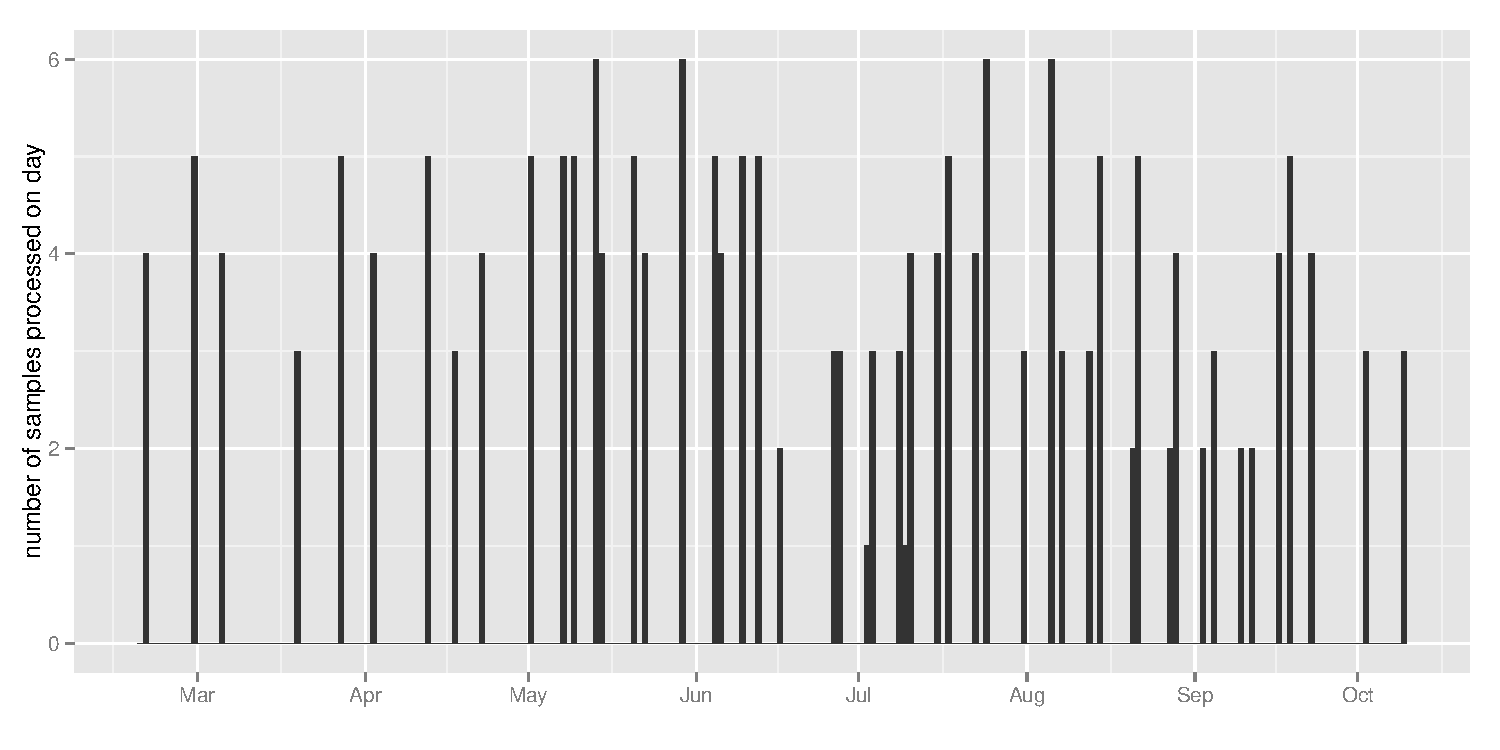
\includegraphics[scale=.5] {flowdatasets/figures/il2ra-samples-time.pdf}
\mycaption{figure:IL2RA-sample-time} 
{Number of samples analysed per day.}
{
A total of 195 (180 + 15 repeats) samples were analysed over seven months (from March to October).
During that period, samples were analysed on $51$ days,
with between one and six samples analysed each day.
}
\end{figure}


\begin{figure}[h]
\centering
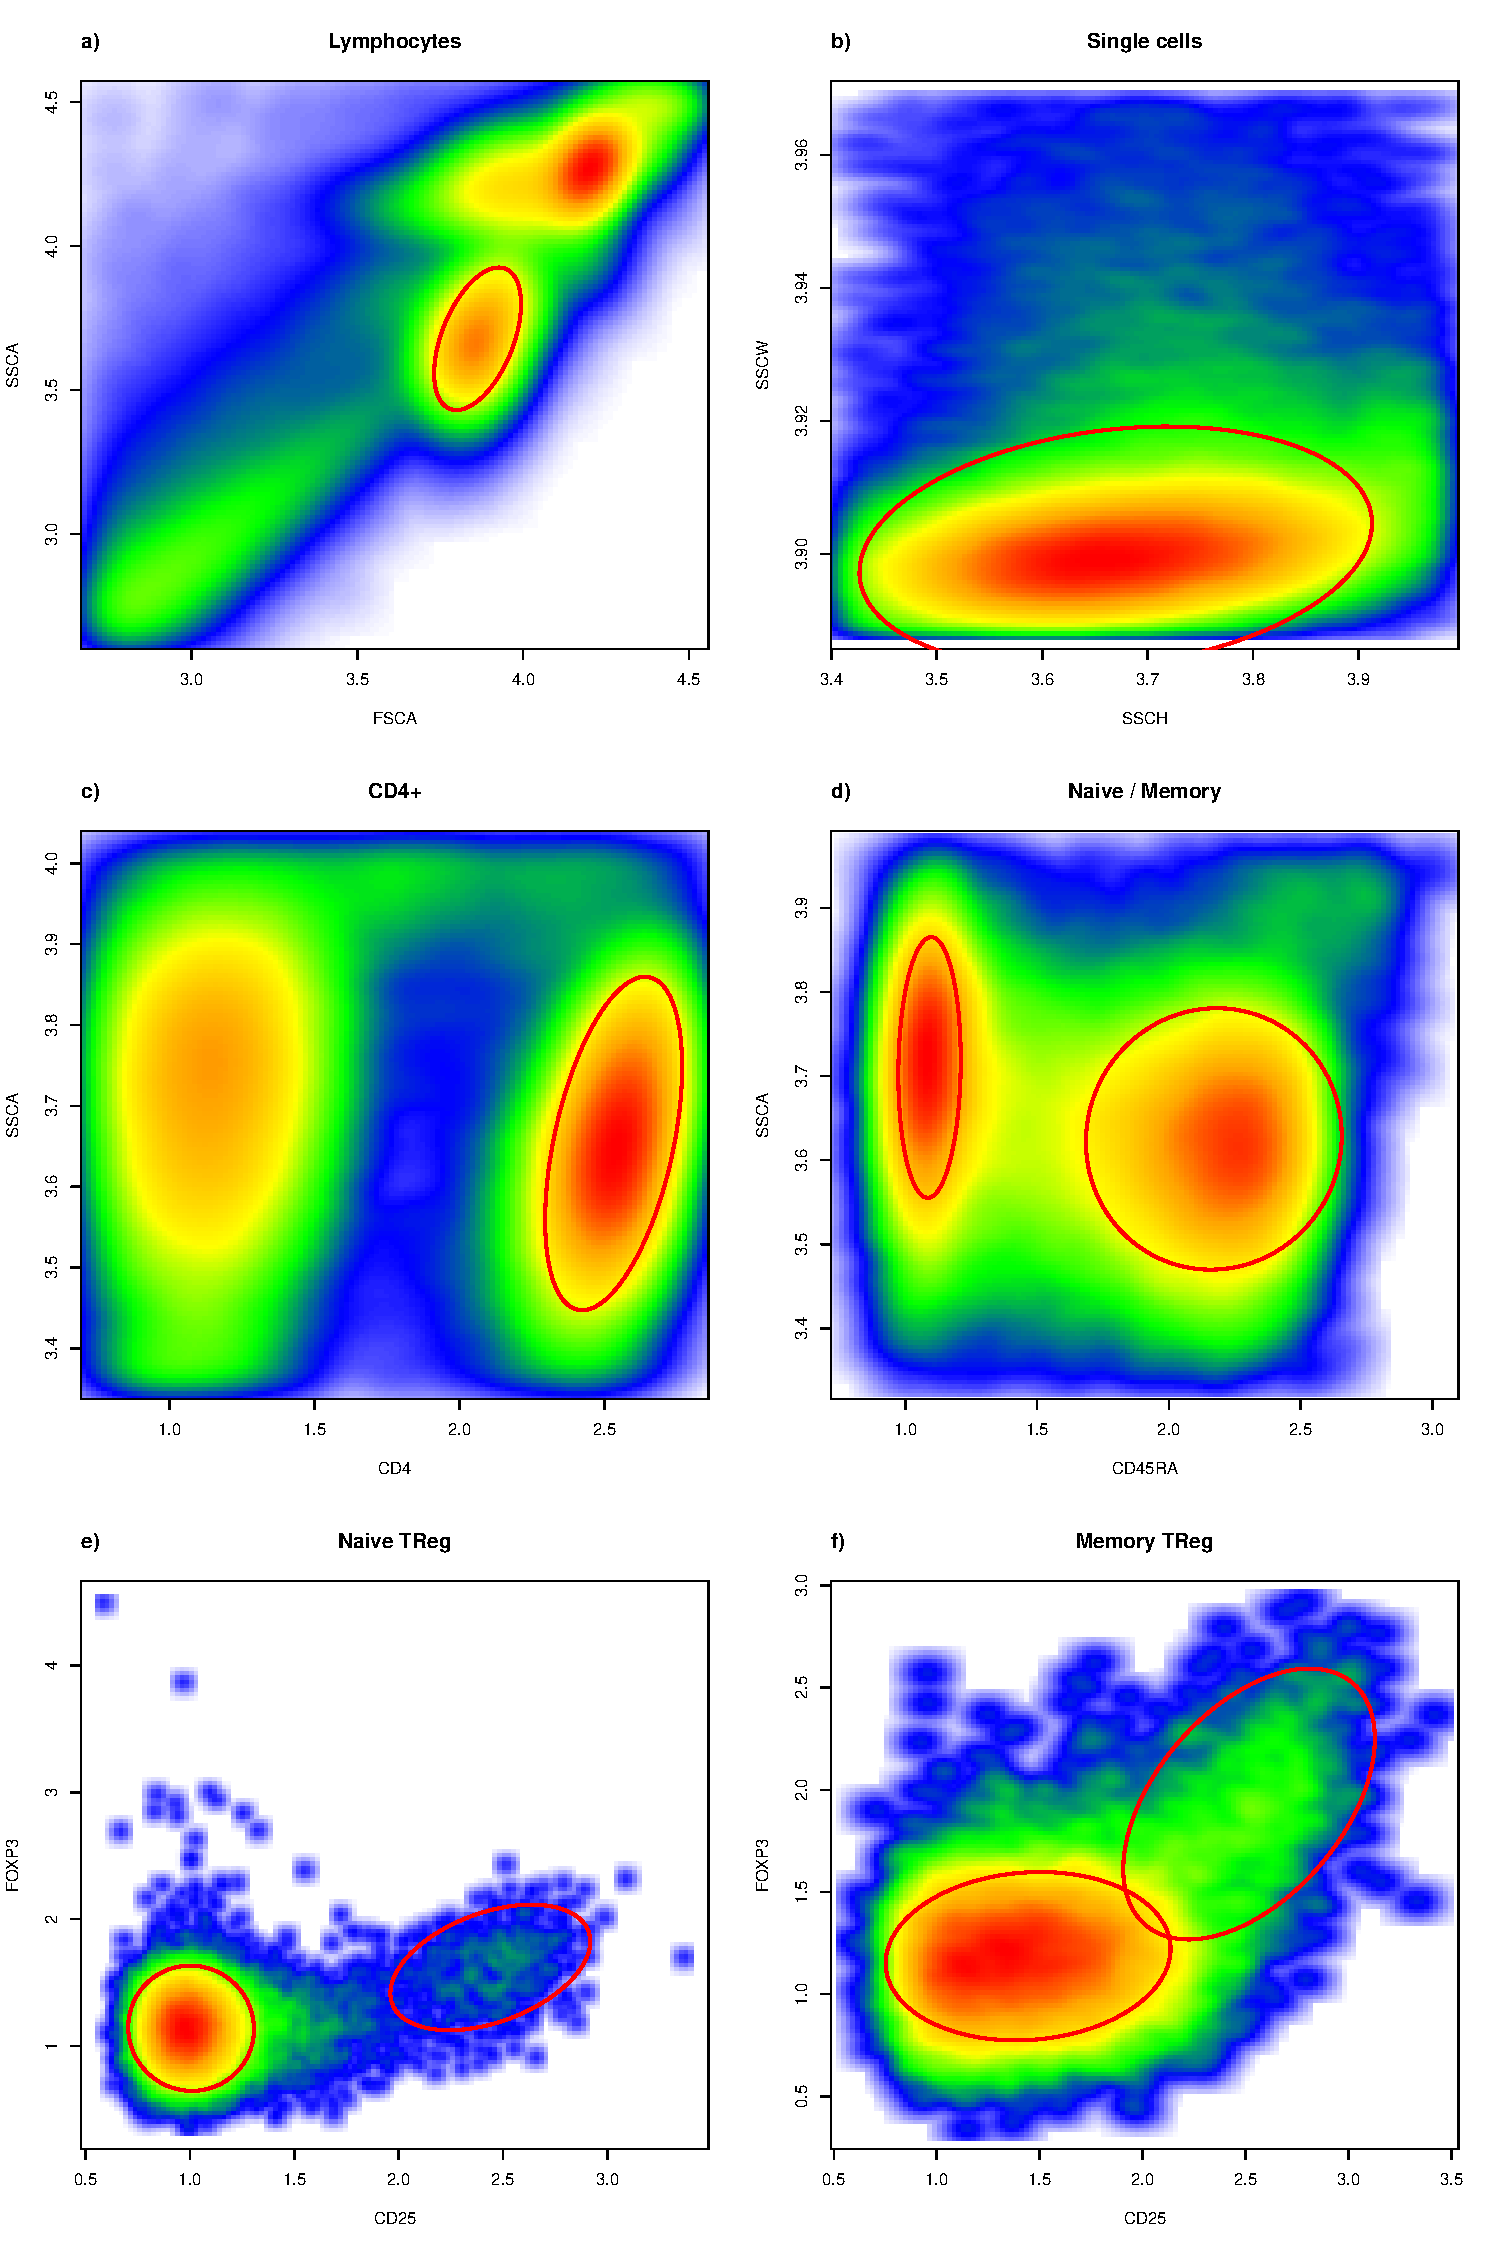
\includegraphics[scale=.5] {IL2RA/figures/ManualGating/manual-gating.pdf}
\mycaption{figure:manual-gating-strategy} 
{Manual gating strategy followed by \citet{Dendrou:2009dv}.}
{
Manual gating strategy to extract memory T cells and CD25\positive naive T cells (green boxes).
Note that the CD45RA gates exclude cells which are considered to be neither memory nor naive.
Our automated gating replaces the final stage of the manual gating on CD25 and CD45RA.

}
\end{figure} 

The cell phenotypes studied by \citet{Dendrou:2009dv}, were obtained using manual gating with the FlowJo software\footnote{\url{www.flowjo.com}}.
Manual gating follows the current state of knowledge of immune cell lineages and the gating strategy followed by \citet{Dendrou:2009dv} is described in \Cref{figure:manual-gating-strategy}.  
Lymphocytes are distinguishable from more granular and larger cell types based on forward and side scatter (\Cref{figure:manual-gating-strategy}a).
The lymphocytes include, B cells and T cells, and the latter population includes cells expressing \protein{CD8} or \protein{CD4}.
Within the lymphocytes, the subset expressing \protein{CD4} are defined as T lymphocytes (\Cref{figure:manual-gating-strategy}b).
The \protein{CD4}\positive T lymphocyte subset can be further divided into regulatory and non-regulatory cells.
Regulatory cells represent a low-frequency subset which has the highest CD25 expression compared to other resting cells, and which
expresses no or very low level of \protein{CD127}.  
%higher in \protein{CD25} and lower in \protein{CD127}.
Regulatory T cells can be defined more precisely by the intracellular \protein{FOXP3} transcription factor, which is constitutively expressed
only in regulatory T cells.
Non-regulatory T cells represent a larger proportion of T lymphocytes,
they express more \protein{CD127} and less \protein{CD25} than regulatory T cells (\Cref{figure:manual-gating-strategy}c).
Non-regulatory T cells can be further divided into naive and memory subsets (\Cref{figure:manual-gating-strategy}d).  
Upon antigen presentation, naive cells are activated and differentiate into effector cells, some of which further differentiate into memory cells
while the remainder die.
%Thus cells are in a transitional state between naive and memory.  
As part of the transition process from naive to memory, the cell surface protein \protein{CD45RA} is lost so that consequently naive cells have higher \protein{CD45RA} expression than memory cells.
A further difference between these subsets is that memory cells tend to have a higher CD25 expression than naive cells.
%A further secondary distinguishable property is that memory cells tend to be higher in \protein{CD25} expression than naive cells.
Since \protein{CD25} expression on the naive cells is low, with only a subset of the cells expressing substantial levels of the molecule,
\citet{Dendrou:2009dv,Pekalski:2013ga} define a threshold above which naive cells are deemed positive for CD25.


% Calli's results
% cell phenotypes
Following this manual gating strategy, two T cell phenotypes, percent of \protein{CD25}\positive naive cells over total naive cell count 
and normalised fluorescence intensity of CD25 on memory cells, were found to be associated with \snp{rs2104286} and \snp{rs12722495} respectively.
The percent of \protein{CD25}\positive naive cells and percent of memory cells, were found to be associated with age and marginally associated with sex.
The repeatability was also tested thanks to the 15 recalled individuals.
Repeatability is an important factor to take into consideration, because reduced within-individual variation increases the power to detect between-individual variation.  
The repeatability and association results, as reported by \citet{Dendrou:2009dv}, are summarised in \Cref{table:calli-results}.  


\begin{table}[h]\footnotesize
\begin{tabularx} {\linewidth} {|XlcXXX|}
\cline{1-6}
\mbox{CD4\positive T Cell} Subset  & Phenotype  & Repeatability ($r^2$) & Genetic Effect                                                            & Age Effect                                & Sex Effect\\
\cline{1-6}
CD25\positive Naive                & Percentage & $0.669$               & \mbox{$\downarrow$ \snp{rs2104286}} \mbox{$\text{P}=4.25 \times 10^{-6}$} & $\uparrow$ \mbox{$P=2.22 \times 10^{-9}$} & \mbox{M < F} \mbox{$P=0.005$}\\
\cline{1-6}
Memory                     & CD25 MEF   & $0.997$               & \mbox{$\uparrow$ \snp{rs12722495}} \mbox{$\text{P}=1.16 \times 10^{-10}$} & None                                      & None \\
\cline{2-6}
                           & Percentage & $0.862$               & None                                                                      & $\uparrow$ \mbox{$P=8.97 \times 10^{-5}$} & None \\
%CD4\positive FOXP3\positive T Cells
%CD25 MEF
%Percentage
\cline{1-6}
\end{tabularx}
\mycaption{table:calli-results}
{Repeatability and significance of effects of percentage of naive \protein{CD25}\positive \protein{CD25} MEF and percentage of memory cell phenotypes.}
{
Subset of results from \citet{Dendrou:2009dv} for cell populations under re-analysis in this chapter.
$r^2$ is the Pearson correlation squared.
}
\end{table}

Besides the genetic and environmental factors driving variation in these cell phenotypes, there are two important sources of technical variation which 
need to be controlled for as they can have some bearing on the repeatability and association statistics:
%staining efficiency, 
instrument variation over time and the subjectivity of manual gating.

\begin{figure}[h]
\centering
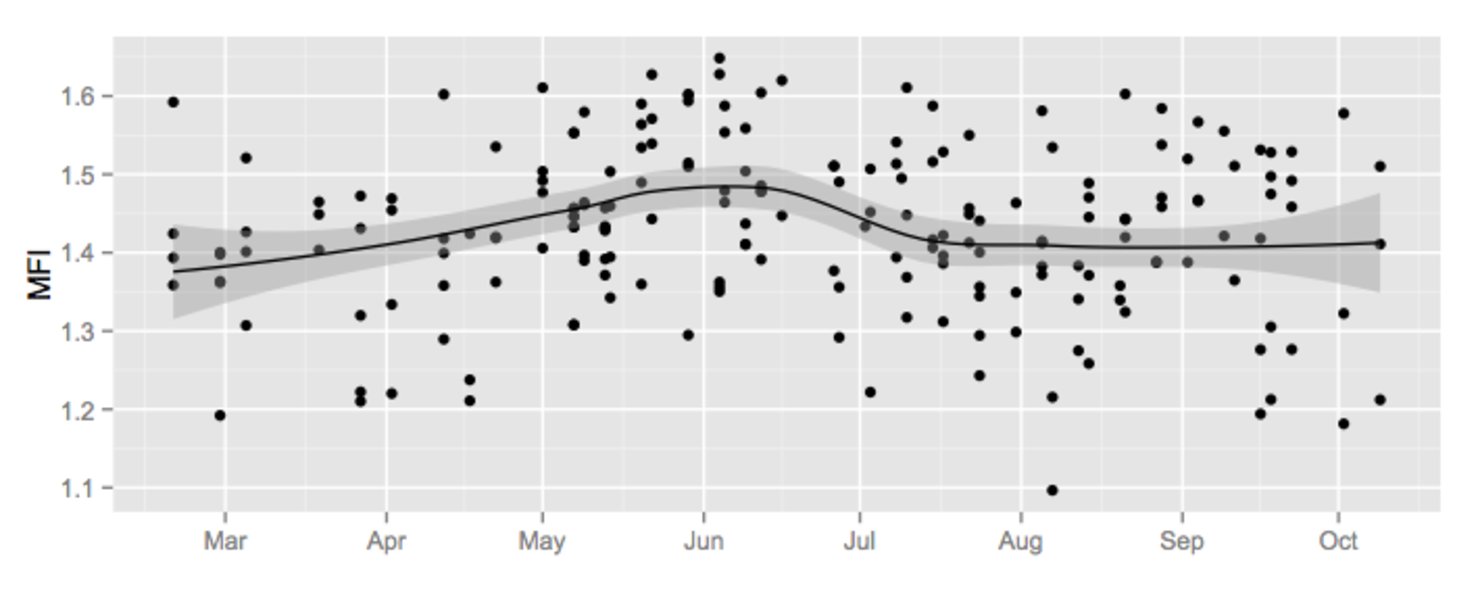
\includegraphics[scale=0.6]{IL2RA/figures/CD25-mfi-time-effect.pdf}
\mycaption{figure:memory-CD25MFI-time-effect}
{Effect of time on CD25 MFI in memory cells.}
{
\protein{CD25} MFI of memory cell population (manually gated) over time of experiment.
The black line represents the loess regression line.
Samples analysed after July tend to have a lower CD25 MFI than those analysed before.
}
\end{figure} 

Over the seven month period of the experiment during which samples were collected and analysed,
instrument variation is detectable in the CD25 \gls{MFI} of the memory cell population (\Cref{figure:memory-CD25MFI-time-effect}).
The influence of this time effect on repeatability was first discussed by \citet{Dendrou:2009bl}.  
To correct for this, \citet{Dendrou:2009dv} run fluorescent six-peak beads daily in order to define a normalisation transform from \gls{MFI} to \gls{MEF}.
Concretely, the transformation is defined by a linear regression
of the observed \gls{MFI} of the six, manually gated, bead populations, against their
expected \gls{MEF}, as specified by the bead manufacturer.
In the first section of the chapter, I will show that this process can be automated by computationally gating beads using my \Rpackage{flowBeads}.

%Next, I will move on to the harder task of algorithmic gating of some 
Manual gating, besides being laborious on large datasets, is an inherently subjective task as it relies on the opinion of the gater and can lead to
between gater variation \citep{Maecker:2005gm}.
Although there is considerable interest in standardising and automating the gating process \citep{Aghaeepour:2013dg},
some customisation is often necessary since some gating steps remains experiment and context specific.  
%This is especially true when defining a positivity threshold on populations which are not clearly bimodal.
For example, when deciding on the position of the CD25\positive gate on the naive cell subset (\Cref{figure:manual-gating-strategy}d), the manual gater 
may rely on fluorescent bead information but also on external experimental information, such as an isotype control.
%a sample not stained with an anti-CD25 antibody but instead with a non-specific antibody conjugated to the same fluorochrome (APC (\Cref{table:IL2RA-panel})), used to assess the background fluorescence.
Nonetheless, I will show, in the second section of this chapter,
that bead data is sufficient in order to develop a computational method which can closely emulate the CD25\positive manual gating.
%even in the absence of isotype controls, a computational method can closely match the CD25\positive manual gating by instead using automatically gated bead data.

%%I will assess, whether I can replicate or improve on these results, with special attention given to repeatability,
%by replacing the last two univariate manual gating steps (Figure 1.2d) with a computational method:
%Univariate gating on CD25 to threshold naive cells into positive and negative subsets, in order to obtain the percentage of CD25+ naive cells.
%Univariate gating on CD45RA to threshold non-regulatory T cells into naive and memory cells, in order to obtain the percentage of memory cells and the CD25 MFI of memory cells.
%Using this method, I will gate \protein{CD25} to threshold naive cells into positive and negative subsets, in order to obtain the percentage of CD25\positive naive cells.  
In the third section of this chapter, I will look at automating the univariate gating on \protein{CD45RA}
in order to identify memory cells.
%to threshold non-regulatory T cells into naive and memory cells.
From this gate, we obtain the percentage of memory cells and the CD25 MFI of memory cells.  
As the CD45RA distribution is typically bimodal, the manual gating of CD45RA into negative (memory) and positive (naive) subsets,
translates well into a clustering problem, which I will attempt to solve by fitting a two-component mixture model.


For both the CD25 and CD45RA gating, I will assess their performance in terms of their repeatability.
%replace the last two univariate manual gating steps (\Cref{figure:manual-gating-strategy}d)
%replacing the last two univariate manual gating steps (Figure 1.2d) with a computational method:
%This method also improves on repeatability.
Finally, in the fourth section of this chapter, I will test the association of the cell phenoytpes, percentage of CD25\positive naive cells, percentage of memory cells and CD25 MEF of memory cells, obtained using these computational methods, in order to assess the influence of these automatic gating approaches on effect size estimation.



%Manual gating follows a step-by-step hierarchical process.
%Ideally the entire manual gating process should be replaced by an automatic algorithm.
%But in order to facilitate initial comparison with manual gating, in this chapter,
%I will only automate the two last univariate gating steps (\Cref{figure:manual-gating-strategy}d):


%adjusted depending on the MFI of the blank beads population on that day.
%\protein{CD25} is known to be upregulated under inflammatory conditions


%CD101,CD127,CD25_MA251+2A3,CD4,CD45RA,HLADR
%CD127,CD25_MA251+2A3,CD4,CD45RA,ISO 



%%% BEADS
\section{Univariate clustering of bead data}

In flow cytometry, a method of normalising fluorescence intensity to account for instrument variation, is to convert the \gls{MFI}
measured on a population to \gls{MEF} \citep{Schwartz:1996jj,Dendrou:2009bl}.
In order to apply this conversion, specially designed beads of known and (assumed) constant fluorescence defined in terms of \gls{MEF}, are used as a reference.
The MEF property of these beads is deemed stable whereas the MFI of the bead population is dependent on the instrument and varies over time.

The beads used here are specially manufactured so that they belong to six distinct populations of increasing MEF as shown in \Cref{table:fluorospheres}.
Following the bead manufacturer's guidelines, plotting the $\log_{10}(MEF)$ of these six bead populations against
the corresponding calculated $\log_{10}(MFI)$ from the gated bead populations, we fit the linear regression:

\begin{equation}
    \log_{10}(\text{MEF})=\beta \times \log_{10}(\text{MFI}) + \alpha
\label{equ:MEF}
\end{equation}

The MEF is in fact a power transform of the MFI (only defined for strictly positive MFI values):

\[
    \text{MEF}= 10^\alpha \times \text{MFI}^\beta
\]

The original MEF transform used by \citet{Dendrou:2009bl} assumes that $\beta=1$,
although I relax that assumption.
%which gives similar results given that I found that the $\beta$ term in \Cref{equ:MEF} turns out to be on average $0.96$.

In calculating the slope $\beta$ and the intercept $\alpha$ parameters of the linear model,
only the five brighest bead populations are used because the MEF of the blank beads is not specified by the manufacturer.
%In fact extrapolating the MEF of the blank beads yields the detection threshold (\Cref{figure:mef}) which we will see in the next section,
However, as we will see in the next section, the blank beads can be used to define a threshold for positivity.
%The MEF of the blank beads is always greater than the intercept $\alpha$  which represents the log offset (the zero channel value).
%Below this threshold the intensity is meaningless as the blank beads contain by design no fluorochrome.

Typically bead data are gated manually.
Here, in order to obtain the parameters of the MEF transform, I will use an automatic process to gate the beads.

Since all beads are manufactured to be of identical dimensions, we expect a single cluster in the scatter channels: the singlet bead population.
Events which lie away from the singlet population are deemed to be beads clumped together or debris and so are discarded.
Filtering of singlets can be achieved by fitting a bivariate normal distribution on forward and side scatter and only keeping
points within the 95th percentile.
Having gated the singlets, I subset the data and proceed to gate on the fluorescence channels to identify the six bead populations.
Given that the number of bead populations is known, that the bead signal is sufficiently clear and that the number of events is small (in the order to 10,000),
I use the K-medoids algorithm (\Cref{appendix:clustering}).
The solution has been implemented in the \Rpackage{flowBeads}, available on BioConductor.
Automatic gating shows near perfect agreement with manual gating (\Cref{figure:bead-agreement}).
%and so is now the established method of analysing bead data in our lab.
Applying the bead normalisation to the memory CD25 MFI from \Cref{figure:memory-CD25MFI-time-effect}, we improve on the repeatability of that 
cell phenotype from $r^2=0.972$ to $r^2=0.985$, where $r^2$ is the Pearson correlation squared (\Cref{figure:CD25-MFI-beads-normalised}).

\begin{table} [hb]
\begin{center}
\begin{tabular} {|c c c c c c|}
\cline{1-6}
Population  & FITC    & RPE     & REP-Cy5 & \textbf{APC}     & PE-Texas Red\\
\cline{1-6}
1           & B       & B       & B       & \textbf{B}       & B \\
2           & 2,500   & 1,500   & 750     & \textbf{4,100}   & 552\\
3           & 6,500   & 4,400   & 2,100   & \textbf{10,300}  & 2,014\\
4           & 19,000  & 14,500  & 6900    & \textbf{25,500}  & 6,975\\
5           & 55,000  & 43,800  & 22,100  & \textbf{67,300}  & 20,685\\
6           & 150,000 & 131,200 & 77,100  & \textbf{139,100} & 71,888\\
\cline{1-6}
\end{tabular}
\end{center}
\mycaption{table:fluorospheres}
{FluoroSpheres from DakoCytomation.}
{
The Molecules of Equivalent Fluorochromes (MEF) values for the six bead populations as provided by the manufacturer.
B denote the blank beads which by design contain no fluorochrome.
Of the six fluorochromes contained by each bead only APC is used in the experiment.
}
\end{table}

\begin{figure}[hb]
\centering
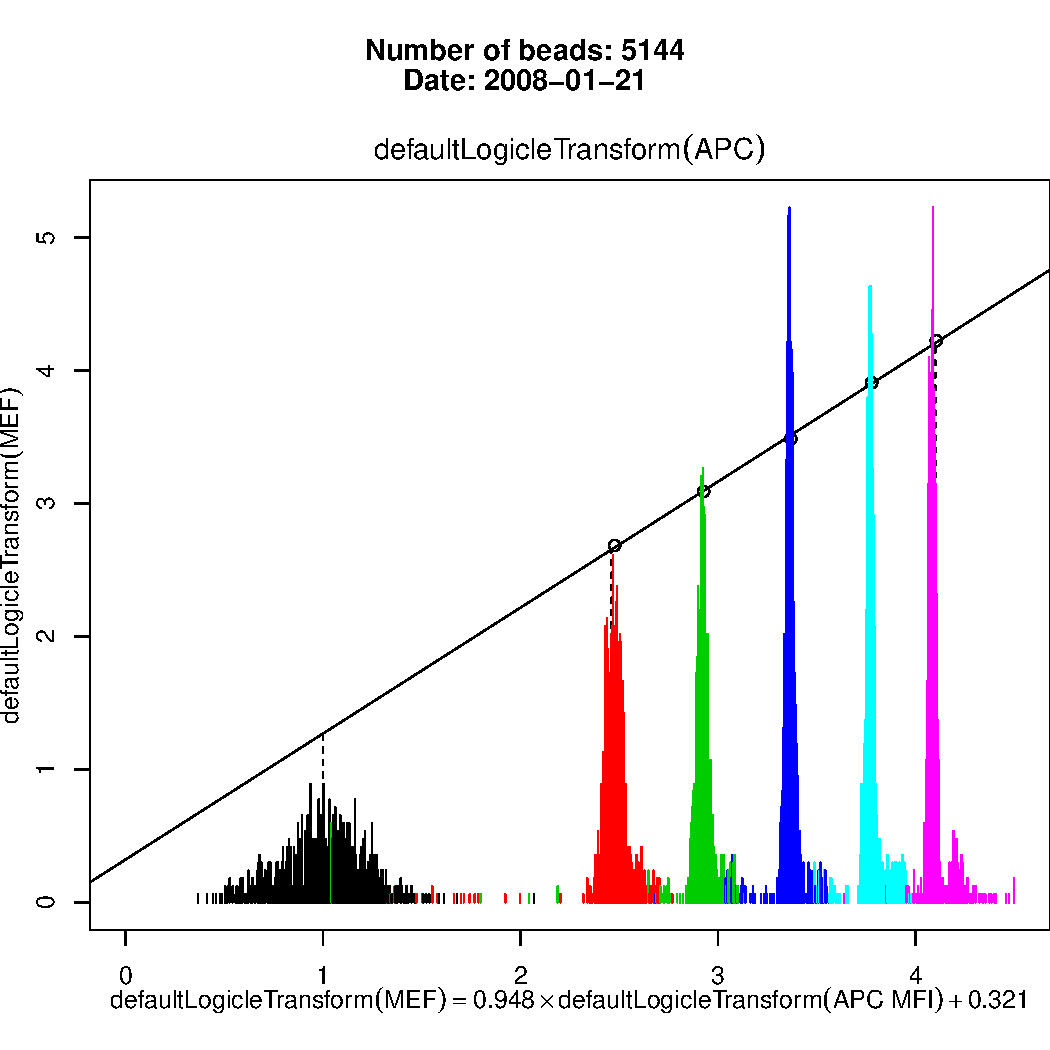
\includegraphics[scale=.5]{IL2RA/figures/Beads/flowBeads.pdf}
\mycaption{figure:mef}
{ Linear regression of bead APC MEF against the APC MFI as defined in \Cref{table:fluorospheres}.}
{
The six peaks represent the six bead populations.
%The horizontal dash lines represent the MEF of the six bead populations.
%The red and green vertical lines define the range of memory CD25 MFI across all samples in \citet{Dendrou:2009dv}.
These types of plots are generated automatically by the \Rpackage{flowBeads}.
}
\end{figure}


\begin{figure}[hb]
\centering
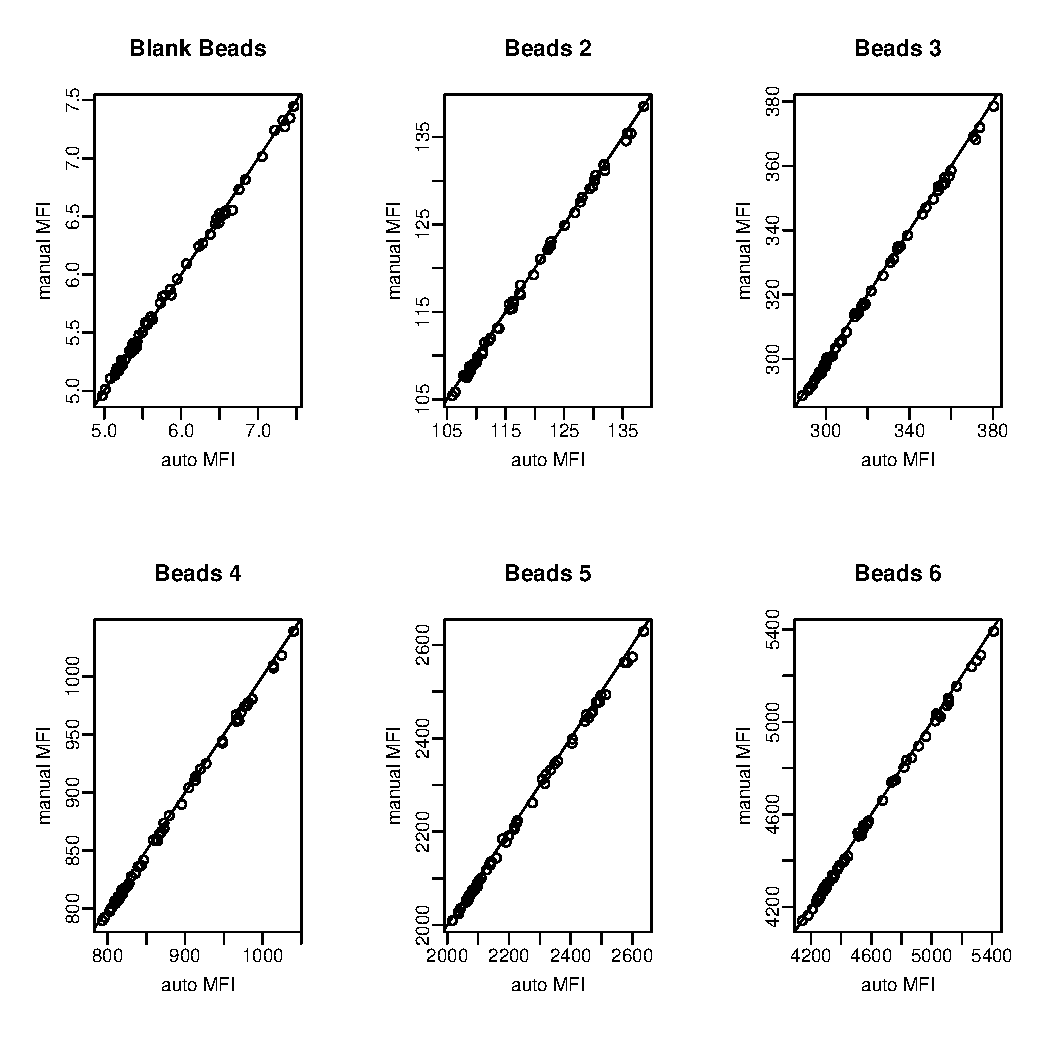
\includegraphics[scale=0.6]{IL2RA/figures/Beads/manual-auto-mfi.pdf}
\mycaption{figure:bead-agreement}
{ Comparison of bead population MFI using manual and \texttt{flowBeads} gating.  }
{ There is good agreement of the APC MFIs of the six bead populations identified with manual and using the automatic approach. }
\end{figure}



\begin{figure}[ht]
\centering
\begin{subfigure}[b]{.4\textwidth}
    \centering
    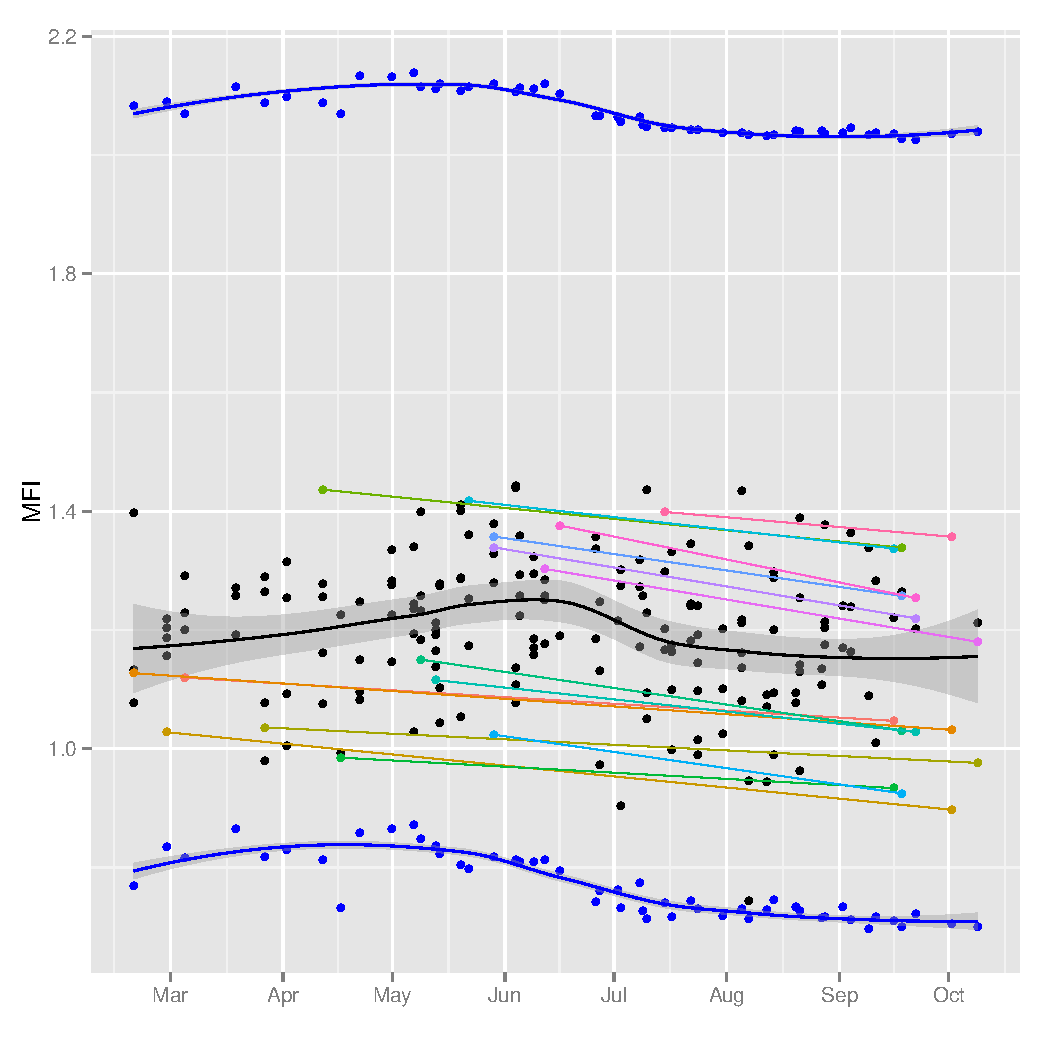
\includegraphics[scale=.3]{IL2RA/figures/CD25-MFI-time-effect-repeatability.pdf}
    \caption{Unormalised}
\end{subfigure}
~
\begin{subfigure}[b]{.4\textwidth}
    \centering
    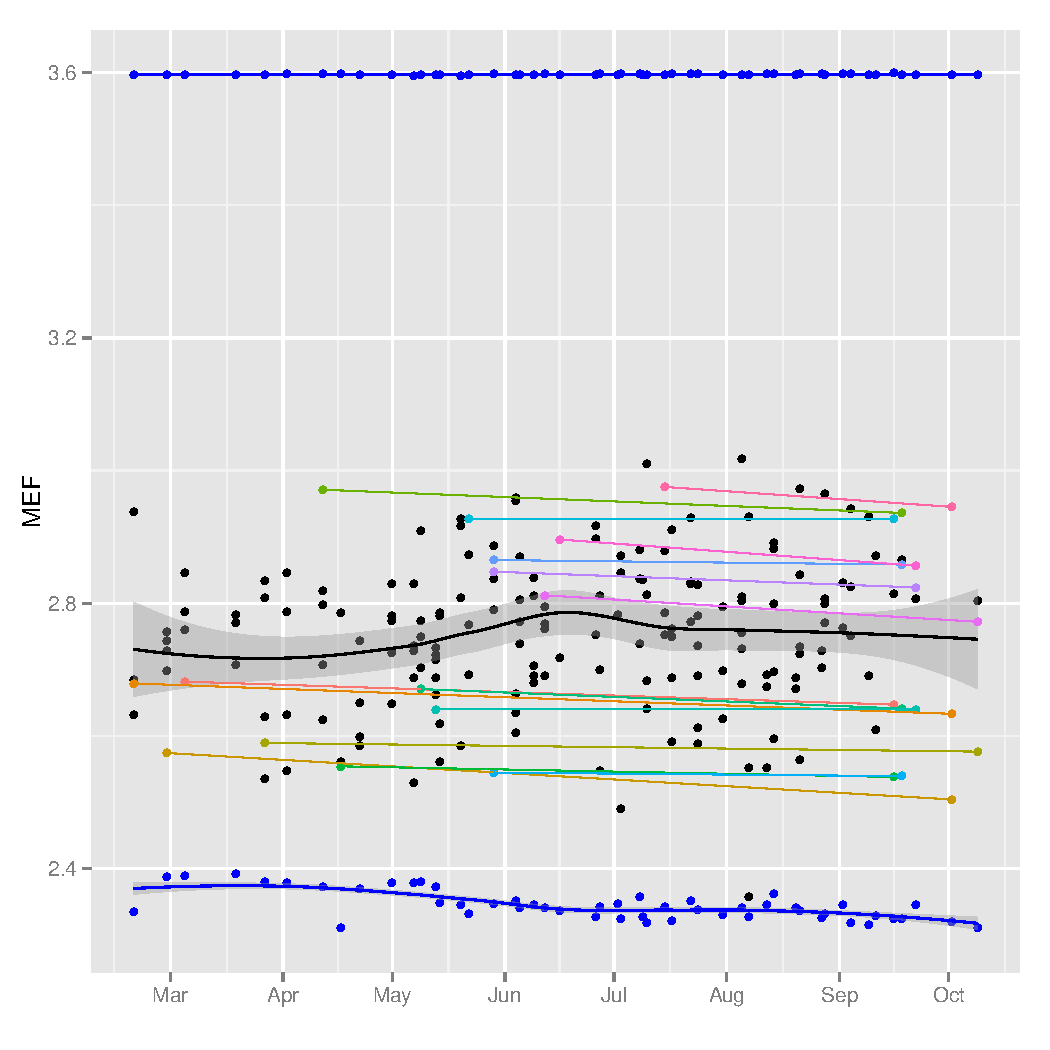
\includegraphics[scale=.3]{IL2RA/figures/CD25-MFI-time-effect-beads-normalised.pdf}
    \caption{Normalised}
\end{subfigure}
~
\begin{subfigure}[b]{.4\textwidth}
    \centering
    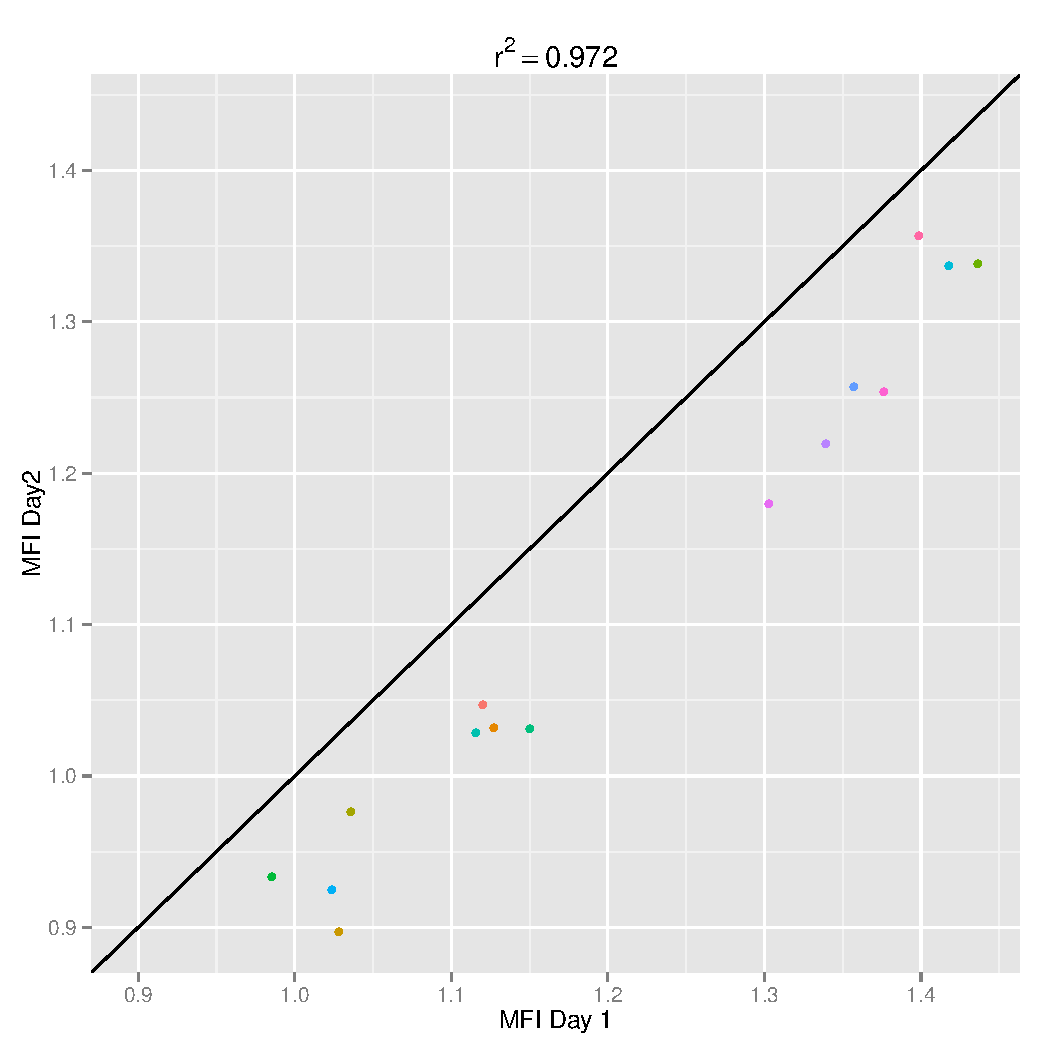
\includegraphics[scale=.3]{IL2RA/figures/CD25-MFI-repeatability.pdf}
    \caption{Unormalised: $r^2=0.972$}
\end{subfigure}
~
\begin{subfigure}[b]{.4\textwidth}
    \centering
    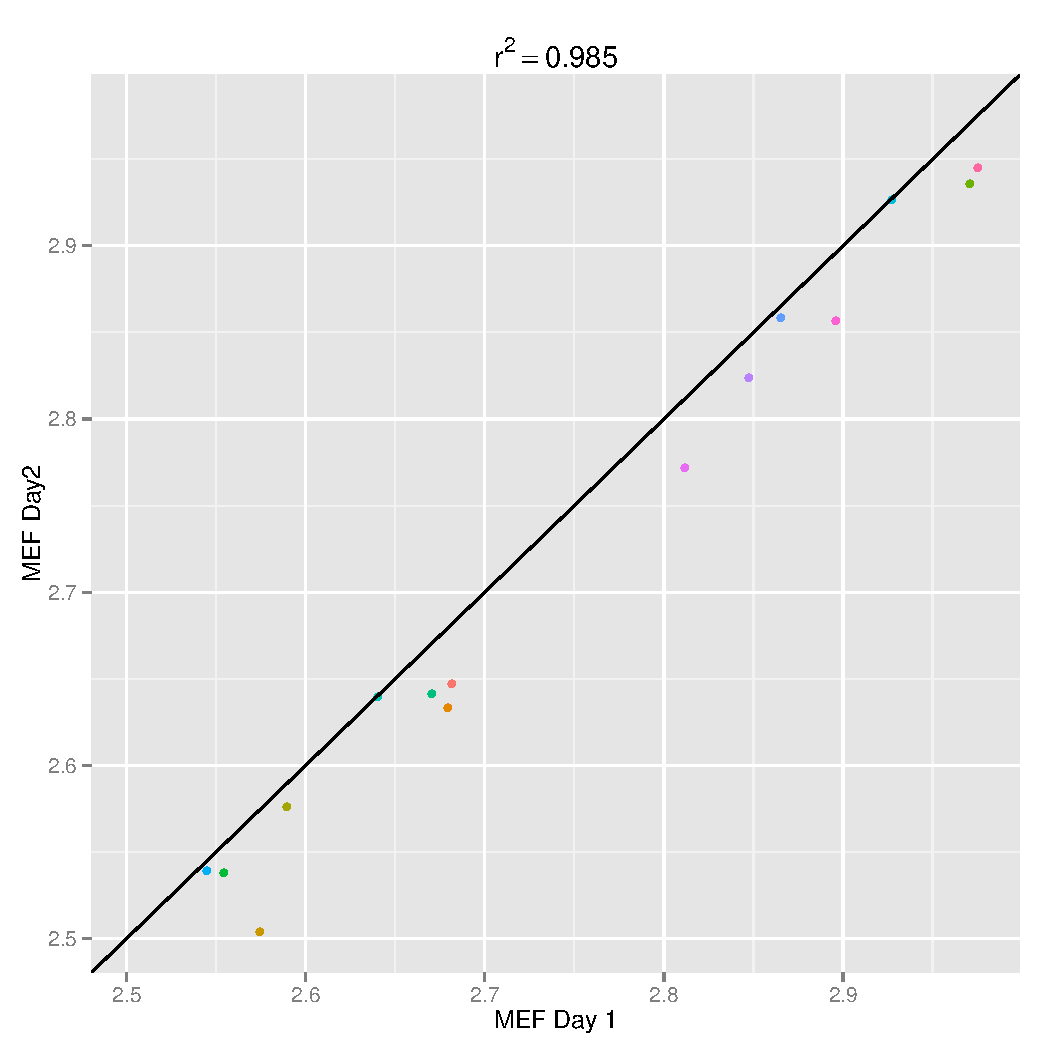
\includegraphics[scale=.3]{IL2RA/figures/CD25-MFI-beads-normalised.pdf}
    \caption{Normalised: $r^2=0.985$}
\end{subfigure}
\mycaption{figure:CD25-MFI-beads-normalised}
{Bead normalisation partially corrects for long term time effect in CD25 MFI of the memory cell population.}
{
  In \textbf{(a)} and \textbf{(b)}, the blue points represent the \protein{CD25} MFIs of the two lowest bead populations,
  in black the \protein{CD25} MFIs of the memory cell populations.
  The dashed blue lines represent the overall mean of each the two bead populations.
  A loess regression is fitted to the MFIs of the beads and memory cells to illustrate the MFI variation over days.
  The points joined by lines are memory cell \protein{CD25} MFIs from the $15$ recalled individuals (\Cref{table:IL2RA-recalled-individuals}).
%The normalisation step involves aligning the peaks of the two bead populations across days to the overall mean of each of the populations (the dashed blue).
  The bead normalisation transform \Cref{equ:MEF} improves the repeatability of the MFI in recalled individuals from $r^2=0.972$ \textbf{(c)} to $r^2=0.985$ \textbf{(d)}.
}
\end{figure}




%%% CD25POS
\section{Univariate gating on CD25: defining a \protein{CD25}\positive threshold on naive cells}

%The population of non regulatory CD4\positive T cells is not clearly bimodal on CD25 like CD45RA.
The approach adopted by the manual method is to define a threshold above which cells are considered positive for CD25.
According to \citet{Dendrou:2009dv} (and \contributor{Calliope Dendrou} personal communication),
the CD25\positive threshold is set manually using an ad-hoc process based on an isotype control, bead data and ultimately a judgement call
by the manual gater.
% already explained in introduction
An isotype control is a sample stained with the same fluorochrome (APC) but conjugated to a
non-specific antibody not designed to target the marker we are interested in quantifying.
It is used as a technique for assessing background APC fluorescence not resulting from CD25 binding.

%These bead populations can also be used to define a threshold above which cells are considered positive for \protein{CD25}, 
%to help overcome the absolute need for isotypes, 
%The threshold for positivity was defined using an isotype control, a sample not stained with an anti-CD25 antibody but instead with an antibody
%with no defined target, conjugated to the same fluorochrome (APC (\Cref{table:IL2RA-panel})).
%The purpose of the isotype control is thereby to observe the background level of any unspecific staining, although
%when dealing with cells with a low Fc receptor expression where unspecific antibody binding is less of an issue.
%Their threshold is defined in terms of an isotype control, a sample not stained for \protein{CD25}, to measure the background.  
%The use of beads can also help overcome the abolute need for isotypes, especially when dealing with cells with a low Fc receptor expression where
%unspecific antibody binding is less of an issue.
%However, even the bead populations themselves require gating, and so in the first section of the chapter...



%adjusted using the daily bead data.
This manual approach to setting the threshold, leads to a different gate position per sample per day (\Cref{figure:cd25pos-gates}).
We notice that on some days there is greater variability in the positions of the gates.
Also, the gate position moves down with time, reflecting the same downwards time-trend in the position of the gates observed in \Cref{figure:memory-CD25MFI-time-effect}.
%which can be explained by position of the gates needing to be shifted down to account for this (\Cref{figure:memory-CD25MFI-time-effect}).

\begin{figure} [h]
\centering
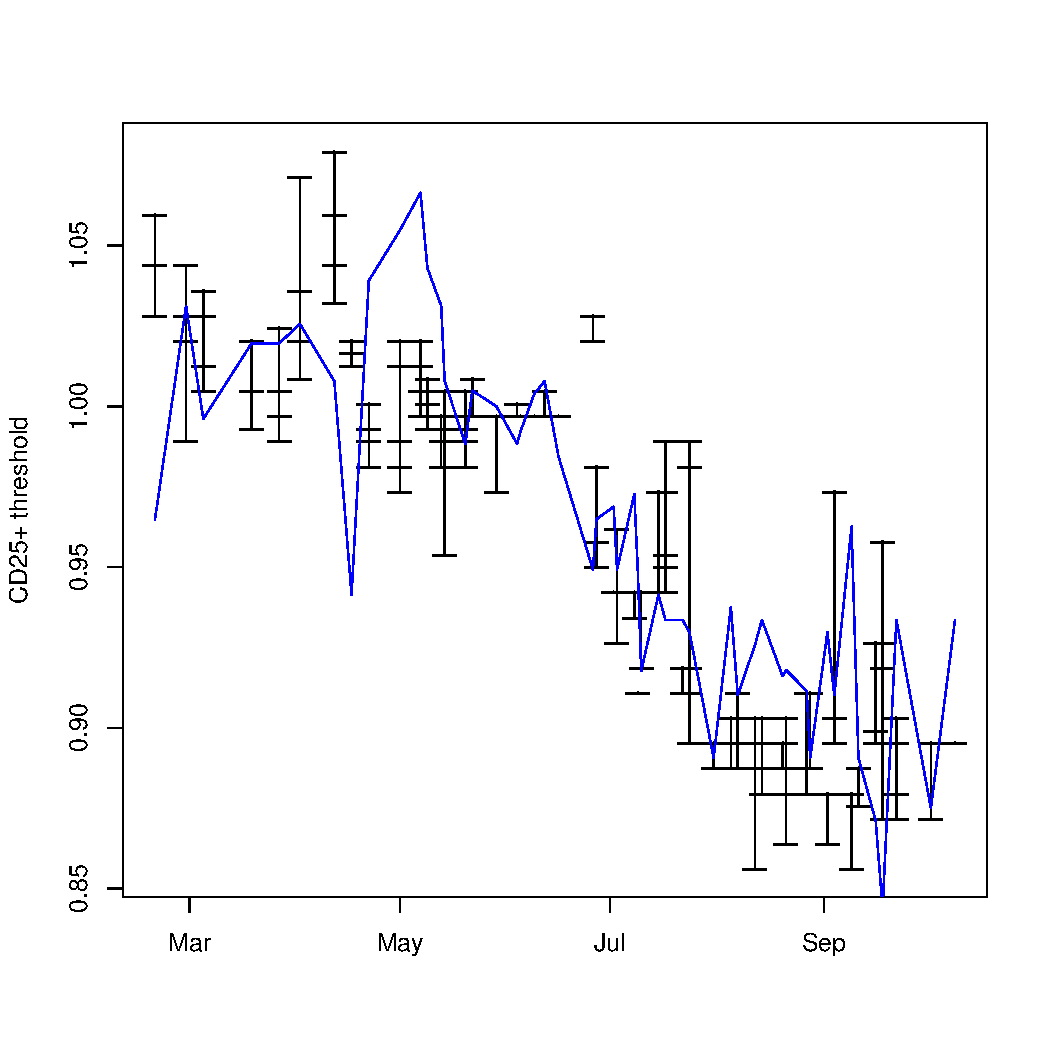
\includegraphics[width=.5\textwidth] {IL2RA/figures/cd25pos-gates.pdf}
\mycaption{figure:cd25pos-gates}
{Position of the \protein{CD25}\positive gate over duration of experiment.}
{
The black horizontal dashes are the positions of the manual CD25\positive gates for all 196 samples over the time course of the experiment (51 days).
The vertical black lines represent the days and so define the range of the manual gate positions on a given day.
The blue line represents our automatic CD25\positive gate which corresponds to the $86^{th}$ percentile of the blank bead population.
}
\end{figure}


%As we can see from \Cref{figure:mef}, the Memory T Cell MFI range is in between the MFI of the blank beads and dimmest bead population.
%Our automatic approach relies 
%Thus we define a threshold to distinguish CD25\positive from CD25 negative cells using the automatically gated bead data on the day which the sample was ran.
Drawbacks of the manual approach are its lack of consistency and its reliance on isotype controls.
The gating criterion is subject to human judgement and so may not be consistent across samples.
Isotype controls are costly since part of the sample and fluorochromes is consumed for control purposes, consequently they are not always analysed.
Also they are not necessarily an accurate measure of background fluorescence since
they are also a source of noise linked to differences in the constitution of the control sample,
the behaviour of the staining and other sources of technical variation \citep{OGorman:1999vd,Maecker:2006ft}.

I wished to improve on this process by using a more consistent and economical approach, using only beads, which I called \texttt{beads.thresh}.
Instead of using isotype data, my working hypothesis,
was that blank beads would constitute a more stable reference, which could be used to define an APC-CD25 threshold.
To find a suitable bead-derived threshold, I first gated the blank beads using my \Rpackage{flowBeads}, then I searched for the APC percentile of the
blank bead population which best agreed with the manual gate (\Cref{figure:cd25pos-gate-agreement}).
I found that in this dataset, the $86^{th}$ percentile of the blank bead population, best matched the manual gate position.

\begin{figure}[h]
\centering
  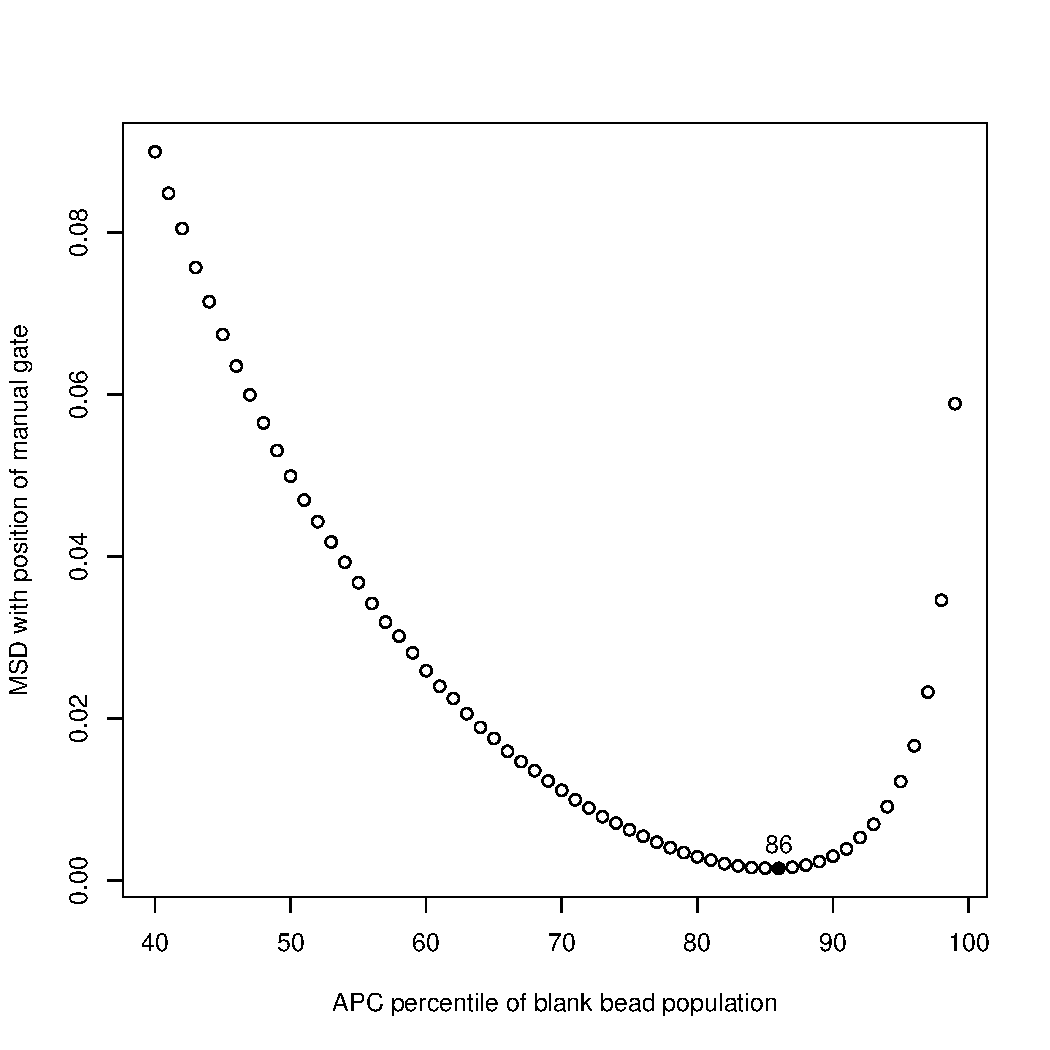
\includegraphics[width=.5\textwidth]{IL2RA/figures/cd25pos-gate-agreement.pdf}
\mycaption{figure:cd25pos-gate-agreement}
%{ Agreement of blank bead derived gate position with manual. }
%{ Comparison of the blank bead derived gate position with the manual equivalent. }
{ Mean square difference (MSD) of the position of the manual gate with that of \texttt{beads.thresh}. }
{
On the x axis, the APC-CD25 percentiles of the blank bead population from 40 to 99.
On the y axis, the mean squared difference between the position of the manual gate and that of the bead-derived gate for that percentile threshold.
The $86^{th}$ percentile yields the lowest mean squared difference hence the best agreement with the manual gating.
The automatic threshold selection method (\texttt{beads.thresh}) is therefore defined as the APC $86^{th}$ percentile of the blank beads population.
}
\end{figure}

\begin{figure}[h]
\centering
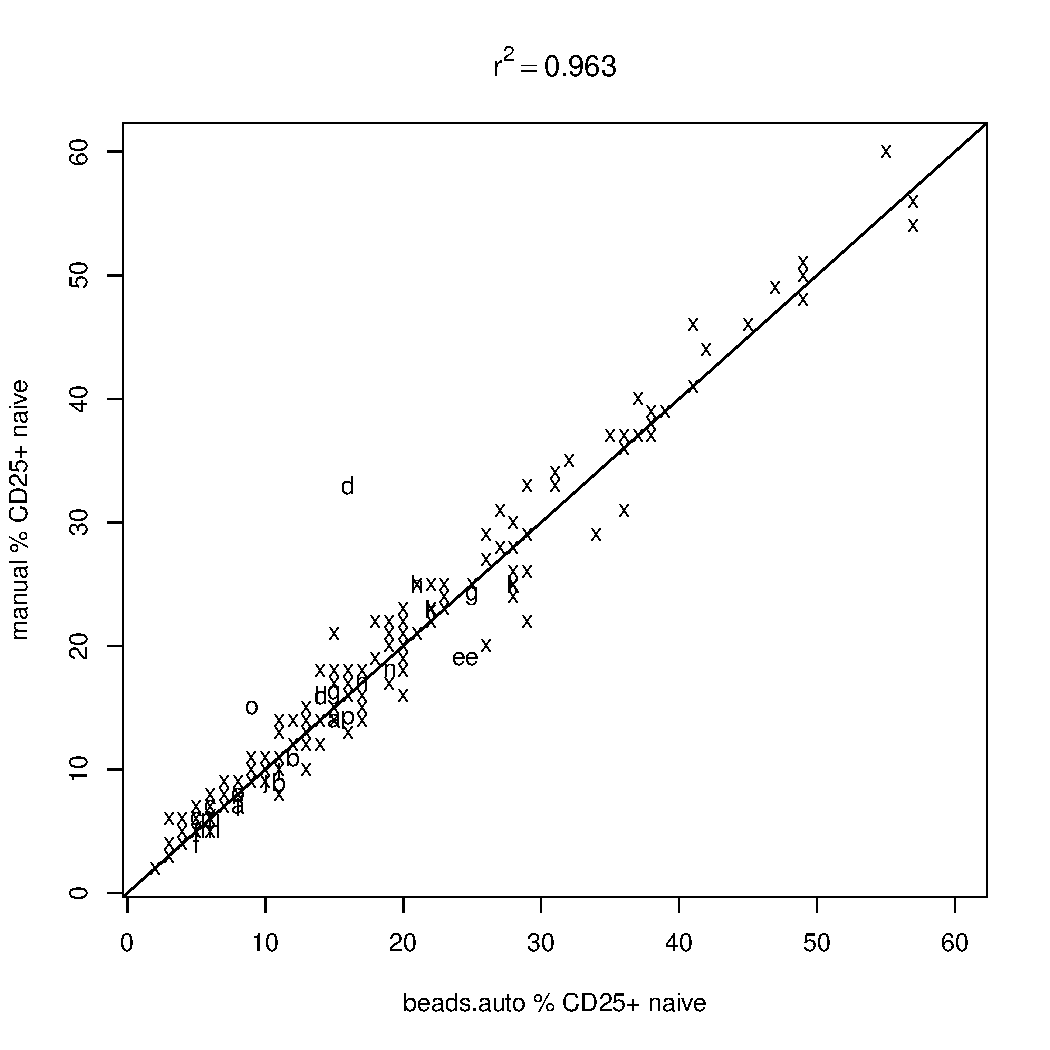
\includegraphics[width=.5\textwidth]{IL2RA/figures/naive-cd25pos-beads-manual-agreement.pdf}
\mycaption{figure:threshold-manual-agreement}
{ Agreement with manual of percentage of \protein{CD25}\positive naive cell phenotype. }
{
  Except for individual d, the agreement of \texttt{beads.thresh} with manual for percentage of CD25\positive naive cells
  is very good.  $r^2$ is the Pearson correlation squared.
}
\end{figure}

Hence the CD25\positive threshold defined by my approach, \texttt{beads.thresh}, is set as the $86^{th}$ percentile of the automatically gated blank bead population on that day.
As we only have one bead set per day, we have a single fixed CD25 gate for all samples on that day (\Cref{figure:memory-CD25MFI-time-effect}).

%In order to assess the dependency of the repeatability on the gates we chose the percentage phenotypes rather than the MEF.
%The concept of repeatability is explained in Appendix~\Cref{repeatability}.
The \texttt{beads.thresh} method for setting \protein{CD25} thresholds  shows improved repeatability of the percentage of \protein{CD25}\positive naive T cell phenotype
over manual (\Cref{figure:repeatability-cd25pos-naive}).  

%One question that might be expected is what would happen if you used automated gating on the isotype and then effectively applied that to the CD25-stained samples?
%A skeptic could argue that  isotype controls might look a bit more variable but that is because they are capturing sample-specific difference, which the beads of course cannot do.
%I'm not saying that I necessarily buy that argument are that you would need to do any further analysis, but I guess it is still a valid question to be aware of.


\begin{figure}[h]
\centering
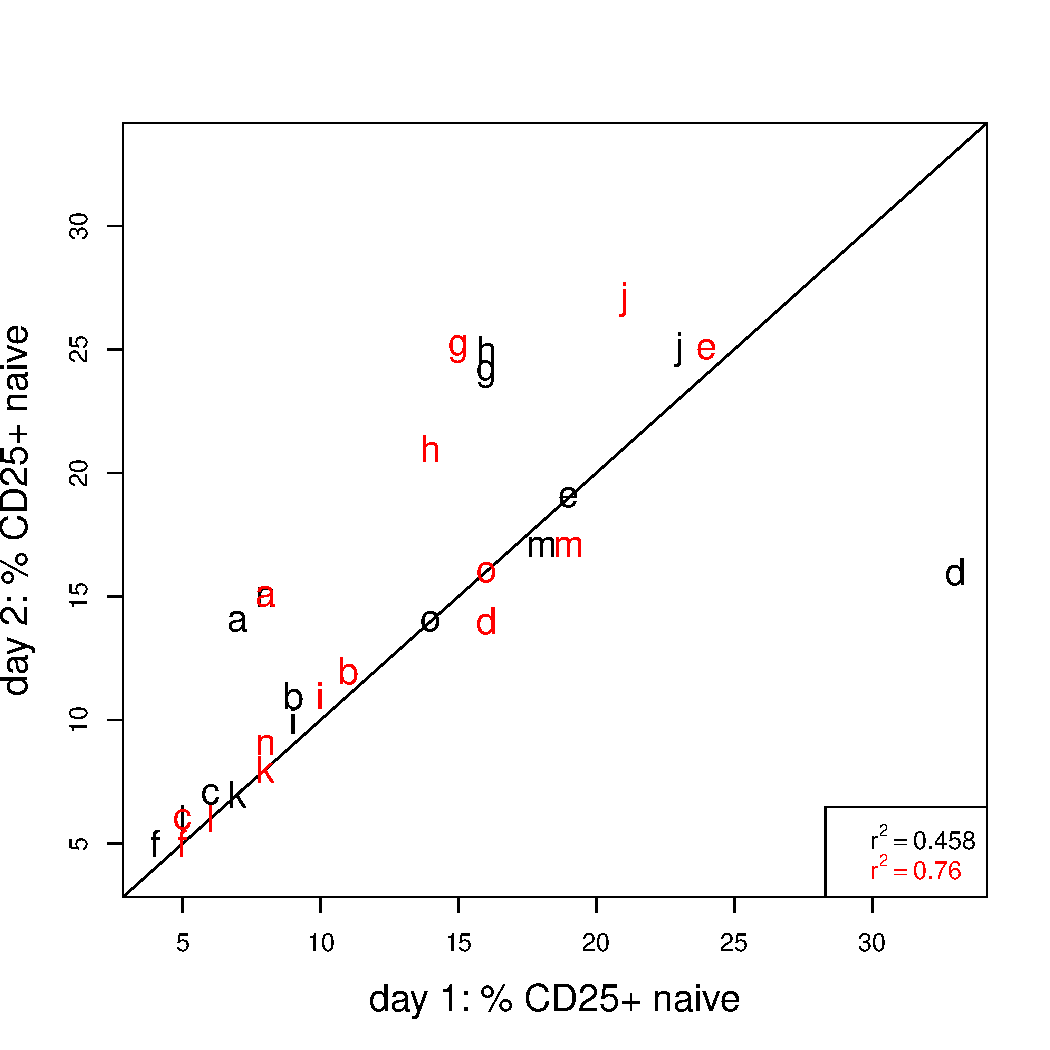
\includegraphics[width=.5\textwidth]{IL2RA/figures/repeatability-cd25pos-naive.pdf}
\mycaption{figure:repeatability-cd25pos-naive}
{ Repeatability of percentage of naive \protein{CD25}\positive with manual (black) and \texttt{beads.thresh} (red). }
{
Repeatability of the percentage of naive cells which are CD25\positive from day one to day two.
The overall repeatability of this cell phenotype was better with \texttt{beads.thresh} (red)
than the manual (black).
Letters are used to identify indidividuals, see \Cref{table:IL2RA-recalled-individuals}.
The Pearson correlation squared is $r^2=0.458$ for manual and $r^2=0.76$ for \texttt{beads.thresh}.
}
\end{figure}

\clearpage

%%% CD45RA
\section{Univariate gating on CD45RA: fitting two-component mixtures on non-regulatory T cells}

Non-regulatory CD4\positive T cells appear bimodal with respect to CD45RA expression,
because this marker is lost upon activation of naive cells (CD45RA\positive) to memory cells (CD45RA\negative).
In this section, we will model the CD45RA distribution by fitting a two component mixture model.
Although we model both populations, we will only gate the memory (CD45RA\negative) cell population, which corresponds to the first component,
since the naive (CD45RA\positive) cell population, the second component, is not a terminal gate as
it is further divided into CD25 negative and positive subsets (see previous section).


%First, I will try a two univariate Gaussian distributions, then I will try a more flexible mixture of two symmetric distributions.
%To this purpose, I used the \Rpackage{mixtools}  which provides an implementation of the \Gls{EM} algorithm \citep{Dempster:1977ul}
%to fit Gaussian (\Rfunction{normalmixEM}).
In order to model the bimodal CD45RA distribution, I use the \Rfunction{normalmixEM} function in the \Rpackage{mixtools},
which provides an implementation of the \Gls{EM} algorithm \citep{Dempster:1977ul}.
The parameters, mean, variance and component weight, of the two-component Gaussian mixture model,
are first initialised by the K-medoids algorithm (Appendix \Cref{appendix:clustering}).
The parameter estimates are then obtained  by running the EM algorithm until convergence.
I call this method \texttt{mm}.
%Because we are only dealing with a mixture of two distributions only one mixing parameter needs to be estimated since the other is simply its complement.
%The other parameters to be estimated are the parameters of the distribution such as the mean and the variance when fitting a mixture of Gaussians or simply the location parameter
%for the semi-parametric distributions..
%More general distributions which are also symmetric
%Semiparametric symmetric distributions are kernel density estimates centered around a location parameter.
%The bandwidth parameter of the kernel density estimate is fixed to $0.1$ but could also have been estimated heuristically from the data.

\subsection{Using the mixing proportions of the mixture model}

Since we are fitting a mixture model, instead of emulating manual gating by picking a threshold,
I will first try a more statistically intuitive approach, using the mixing proportions obtained from \texttt{mm}.
Additionally to the \texttt{mm} approach, I will also apply a more flexible mixture model of semi-parametric symmetric distributions (\Rfunction{spEMsymloc}) again from the \Rpackage{mixtools}, which I will call \texttt{spmm}.
%Returns semiparametric EM algorithm output (Bordes et al, 2007, and Benaglia et al, 2009) for location mixtures of univariate data and symmetric component density.
%The other parameters to be estimated are the parameters of the distribution such as the mean and the variance when fitting a mixture of Gaussians or simply the location parameter
%for the semi-parametric distributions..
%More general distributions which are also symmetric
Semiparametric symmetric distributions are kernel density estimates centered around a location parameter.
%The bandwidth parameter of the kernel density estimate is fixed to $0.1$ but could also have been estimated heuristically from the data.

Comparing the percent of memory cell obtained using \texttt{mm} and \texttt{spmm} to those obtained using manual (\Cref{figure:agreement-memory-weights}), we see that
although there is agreement between the methods, the automatic methods tend to underestimate the percentage of memory cells.
%Check that this not because of zero value intensity not being re-added
Also with regards to repeatability, \texttt{mm} and \texttt{spmm}, yield worse repeatability than manual (\Cref{figure:repeatability-memory-weights}).
%As is the case for the sample from individual d on day one (\Cref{figure:cd45ra-threshold-example}),
%the repeatability is compromised when the mixture of distributions approach fails to find a suitable gate because of poor model fit.

%As the same individual shows a very different profile on day two, I believe that, in this case, the noise is due to technical variation on that day rather
%than true biological variation.
%\subsection{Improved Repeatability when Averaging Gate Positions}


\begin{figure}[h]
\centering
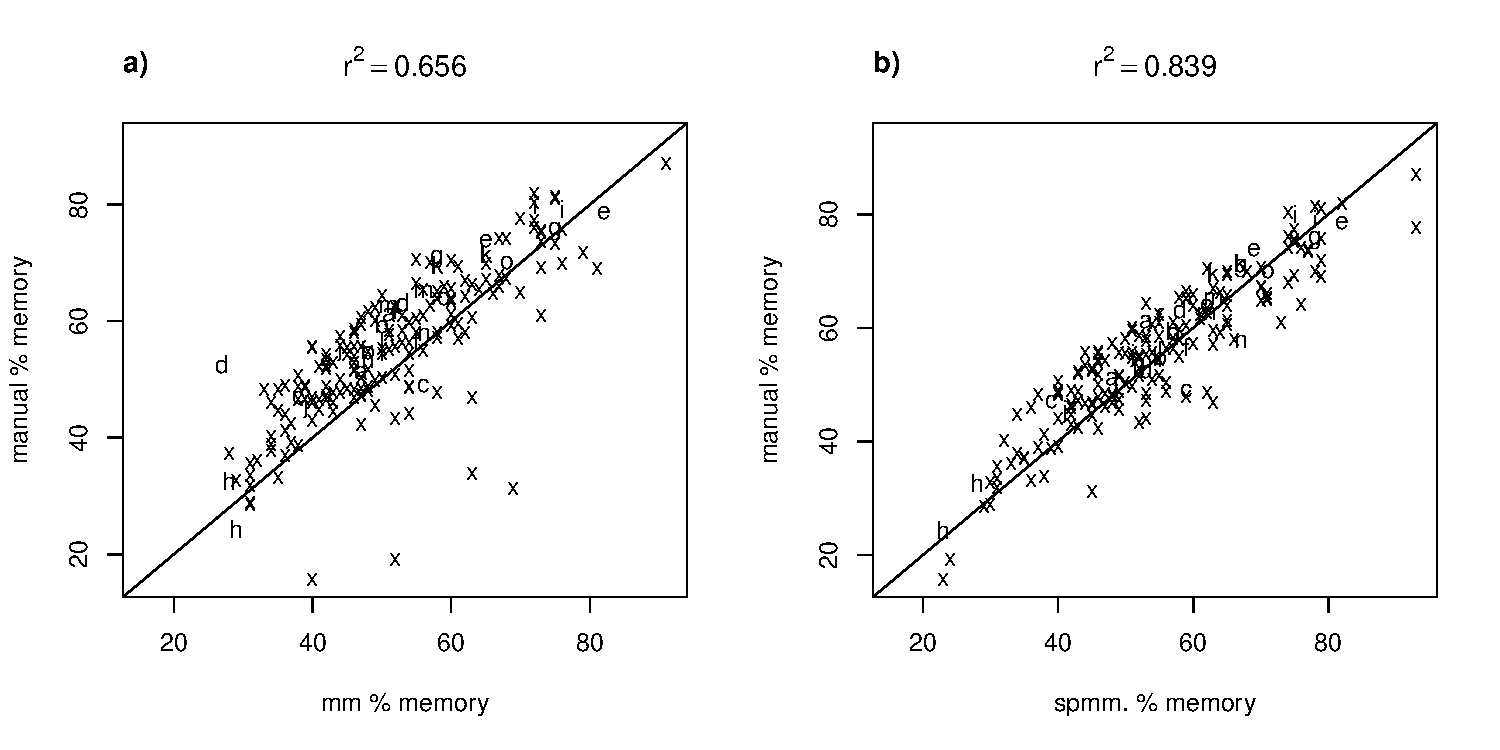
\includegraphics[scale=.5]{IL2RA/figures/memory-auto-manual-agreement-weights.pdf}
\mycaption{figure:agreement-memory-weights}
{Agreement with manual of the percent memory cell phenotype obtained with \texttt{mm} (a) and \texttt{spmmm} (b).}
{
  The more flexible model, \texttt{spmm}, tends to agree better with percent memory cell phenotype returned by manual, than \texttt{mm}.
  %\texttt{mm} tends to report a higher percentage of memory cells than reported by manual.
  Again we can see in (a), that \texttt{mm} underestimates the percentage of memory cells in individual d compared to
  manual.

}
\end{figure}


\begin{figure}[h]
\centering
  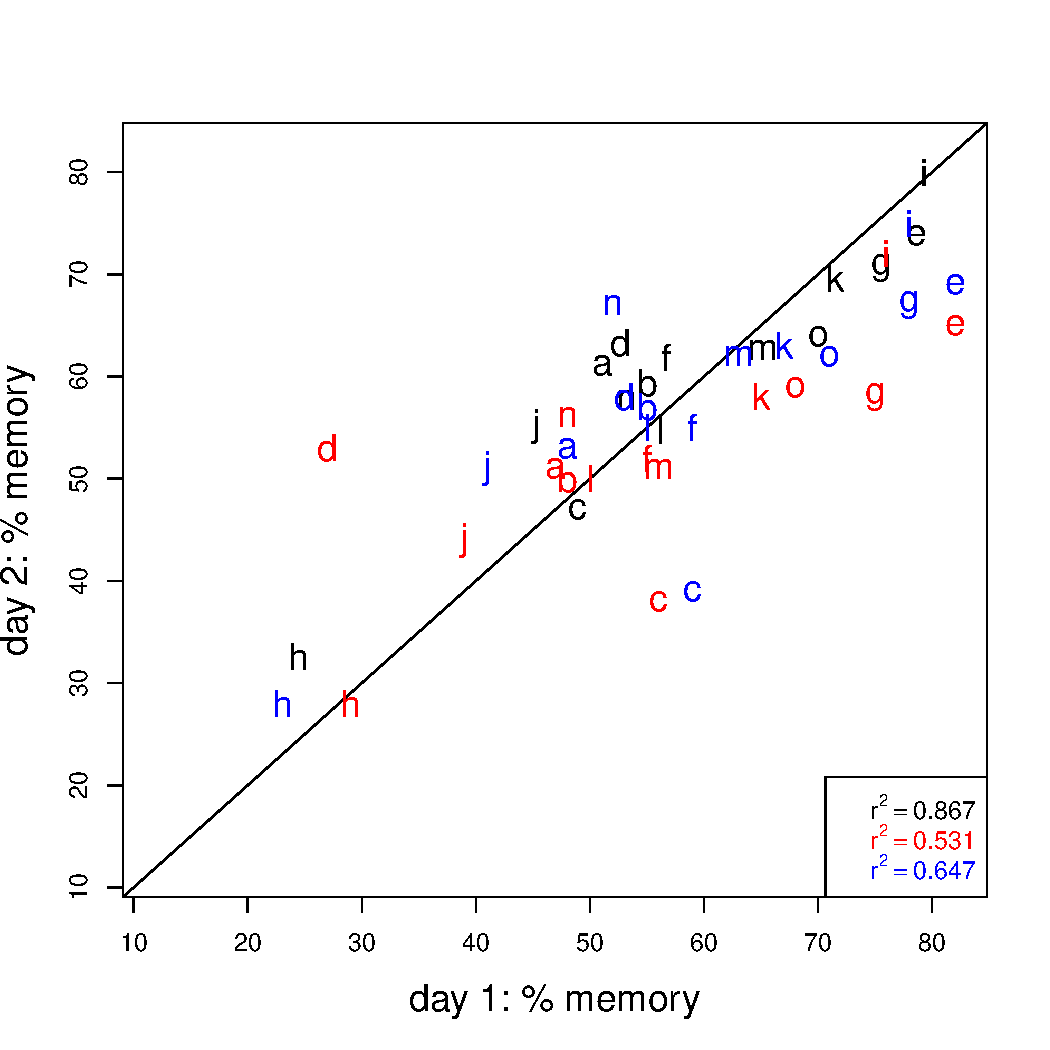
\includegraphics[width=.5\textwidth]{IL2RA/figures/repeatability-memory-weights.pdf}
\mycaption{figure:repeatability-memory-weights}
{Repeatability of the percent memory cell phenotype with manual (black), \texttt{mm} (red) and \texttt{spmm} (blue).}
{
  While manual still shows the best repeatability, the repeatability of the automatic methods is quite encouraging, given
  these have no knowledge of the manual gates and are based purely data driven.
  Also as seen using the thresholding methods, individual d is a clear outlier when gated with the \texttt{mm} method.
}
\end{figure}


\subsection{Emulating manual gating by picking a threshold}

Although the previous approach makes sense from a statistical perspective, it does not exclude the transitional cell population which lie
between the memory and naive cells.
Instead in the manual gating, the memory cell subset is defined by a threshold on the bimodal CD45RA distribution, below which cells are regarded as CD45RA\negative.
Here, I attempt to emulate manual gating by defining a threshold on the fitted two-component mixture model, \texttt{mm}.
%later, I will consider using the mixture weights.  
I consider two approaches of selecting a threshold, \texttt{pct.thresh} and \texttt{post.thresh}, both which are illustrated in \Cref{figure:cd45ra-threshold-example}.


\begin{figure}[h]
\centering
  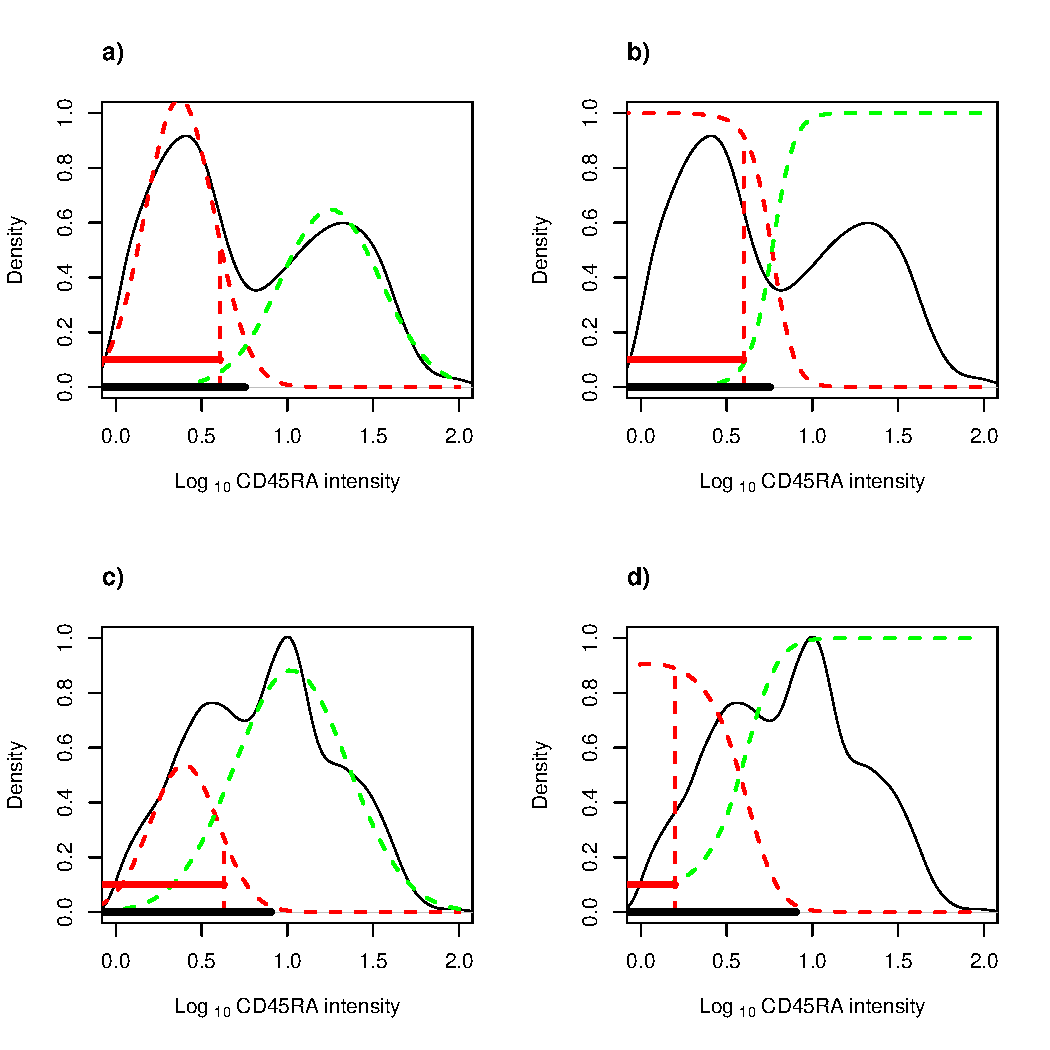
\includegraphics[scale=.6]{IL2RA/figures/cd45ra-threshold-example.pdf}
\mycaption{figure:cd45ra-threshold-example}
{ Example on individual d of the two approaches, \texttt{pct.thresh} (a and c) and \texttt{post.thresh} (b and d), of selecting a threshold. }
{
  Individual d was chosen to illustrate \texttt{pct.thresh} and \texttt{post.thresh}, because
  the CD45RA distribution takes on a very different shape on day one (a and b) compared to day two (c and d).
  In (a) and (c), the \texttt{pct.thresh} method, places the gate at the 88th percentile of the first component.
  In (b) and (d), the \texttt{post.thresh} method, places the gate at the largest CD45RA value where the posterior of the first component reaches 89 percent.
  This poses a problem for \texttt{post.thresh} in (d) because the overlap of the components is such that the posterior is only reached close to zero
  which yields a much smaller gate and consequently a lower percent of memory cells (\Cref{figure:memory-auto-manual-agreement-thresholds}d).
  On the other hand, while the two-component distribution is not a good fit to the data, this is less of an issue for \texttt{pct.thresh}, as can be seen in (c).
}
\end{figure}



\begin{figure}[h]
\centering
  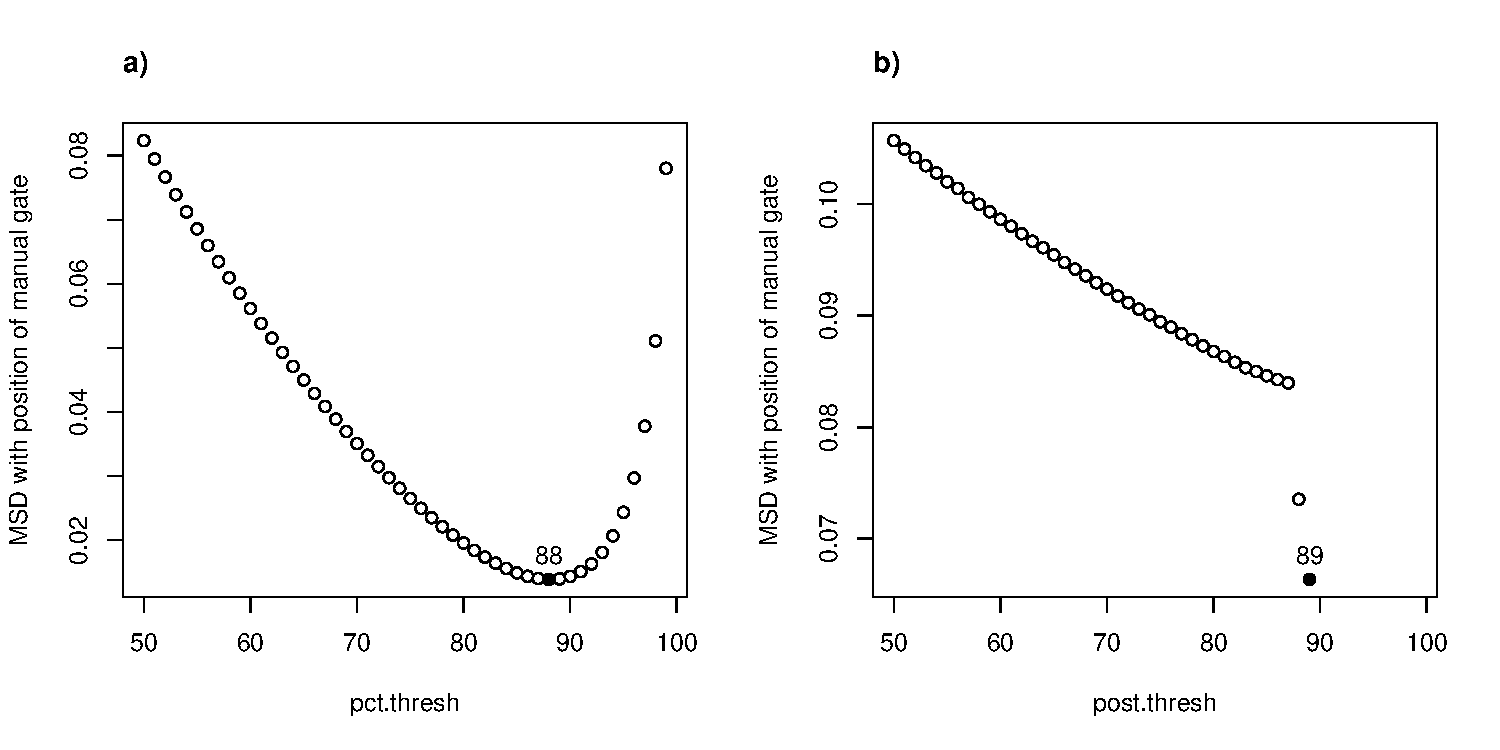
\includegraphics[width=\textwidth]{IL2RA/figures/cd45ra-gate-agreement.pdf}
\mycaption{figure:cd45ra-gate-agreement}
{ Mean square difference (MSD) of the position of the manual gate with that of \texttt{pct.thresh} (a) and \texttt{post.thresh} (b). }
{
  The threshold which minimises the MSD is 88 for \texttt{pct.thresh} (a) and 89 for \texttt{post.thresh}.
  At that threshold, the \texttt{pct.thresh} (a) gate position matches better the manual than \texttt{post.thresh} (b).
  For \texttt{pct.thresh}, the MSD is not defined for threshold larger than 89,
  because there are samples for which the posterior probability does not reach 89 percent (\Cref{figure:cd45ra-posterior-threshold-fail}e).
}
\end{figure}


The first method, \texttt{pct.thresh}, closely replicates the manual CD45RA\negative gating procedure, as explained to me by \contributor{Linda Wicker}.
In this approach, only the shape of the first left-most, component of the mixture model defines the position of the \protein{CD45RA}\negative memory gate.
In order to delineate the memory population, we first identify the first peak of the bimodal CD45RA distribution,
which should correspond to the peak of the first component, after the two-component mixture has been fitted.
Then, following the CD45RA density curve from the peak towards the left-hand-side,
we record the CD45RA value after which the density curve drops below a certain given threshold.
This CD45RA value is then mirrored to the right-hand-side of the peak in order to define the CD45RA- threshold.
This technique is in fact equivalent to selecting a fixed percentile threshold
for the first component to gate consistently across all samples.
%an manual approach to consistently drawing a CD45RA memory gate across all samples 
%is closer to manual gating is to only consider the shape of the memory cell population
%to draw the threshold. Here, a percentile of the first component can be used as cut-off.

The second method, \texttt{post.thresh}, considers the density ratio of both components in order to decide where to draw a threshold.
Formally, \texttt{post.thresh} selects a threshold on the posterior probability of belonging to the first component, the memory population, across all samples.
At a given point, the posterior probability of belonging to the first component is defined as the ratio of the density of the first component,
over that of the total density.
%The posterior probability can be interpreted as the confidence with which an event can be assigned to a component.
Concretely, given a two-component mixture model where, $f_1$ is the density of the first component and $f_2$ the density of the second, and a posterior threshold of $p$,
then a point $x$ is assigned to component 1 provided that:
\[
  f_1(x) \geq f_2(x) \dfrac{p}{1-p}
\]
For example, if the posterior probability threshold was $p=95\%$, then for $x$ to be assigned to the first component, $f_1(x)$ would need to be $19$ times larger than $f_2(x)$.

Given these two thresholding approaches, I wish to select a threshold for \texttt{pct.thresh} and for \texttt{post.thresh}, which most closely matches the manual gating.
To this purpose, I use the method described in the previous section (\Cref{figure:cd25pos-gate-agreement}), to find the threshold which minimises the mean square difference with the manual gate position.
Applying this method, I find that the optimal threshold is the $88^{th}$ percentile for \texttt{pct.thresh},
and $89\%$ for \texttt{post.thresh} (\Cref{figure:cd45ra-gate-agreement}).
Also, I notice that for \texttt{post.thresh}, in certain samples,  the posterior probability
of belonging to the first component does not exceed $89\%$ (\Cref{figure:cd45ra-posterior-threshold-fail}).
This is why in \Cref{figure:cd45ra-gate-agreement}, we do not obtain points beyond a threshold of 89, because gates are missing for certain samples.
This can be due to poor model fit (\Cref{figure:cd45ra-posterior-threshold-fail}a) or too much overlap between the memory and naive cell populations.

\begin{figure}[h]
\centering
  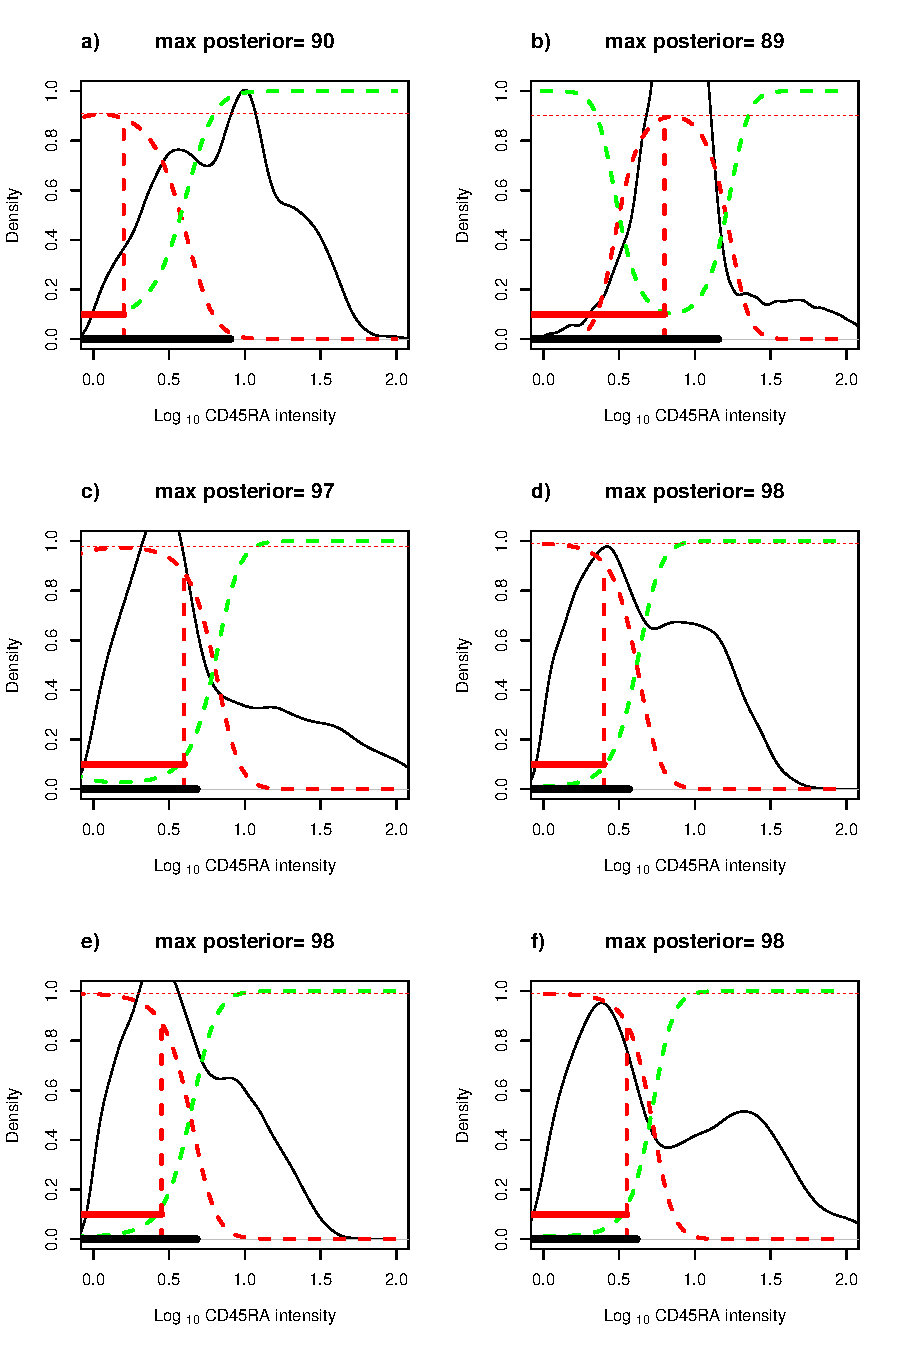
\includegraphics[scale=.6]{IL2RA/figures/cd45ra-posterior-threshold-fail.pdf}
\mycaption{figure:cd45ra-posterior-threshold-fail}
{Samples for which the 99 maximum posterior probability is not reached.}
{
  In black the manual gate.  In red the \texttt{post.thresh} gate drawn at $89$.
  The posterior probability does not reach 99 percent in these six samples.
  In a) this is because of poor model fit.
  In the others b), c) and d), this is due to the mixing of the two distributions.
  In b), the non-uniform decreasing posterior function, can be explained by the green distribution, component 2,
  being much wider than the red distribution.
}
\end{figure}


Using either approach, there is good agreement between the CD25 MEF values obtained for the memory population when gated using either the automated
or the manual approach (\Cref{figure:memory-auto-manual-agreement-thresholds}).
%Using either approach, the agreement with manual gating for the memory CD25 MEF is good (\Cref{figure:memory-auto-manual-agreement-thresholds}).
This is to be expected as this cell phenotype is not very sensitive to the position of the \protein{CD45RA} gate
(\Cref{figure:cd45raneg-memory-cd25mfi}).  
Hence, for this phenotype, this translates to similar repeatability to that obtained with manual gating (\Cref{figure:repeatability-memory-thresholds}).
%and similar effect sizes (\Cref{table:memory-cell-mef-effect}).
On the other hand, the repeatability of the percentage of memory cells is very sensitive to the gate position.


\begin{figure}[h]
 \centering
 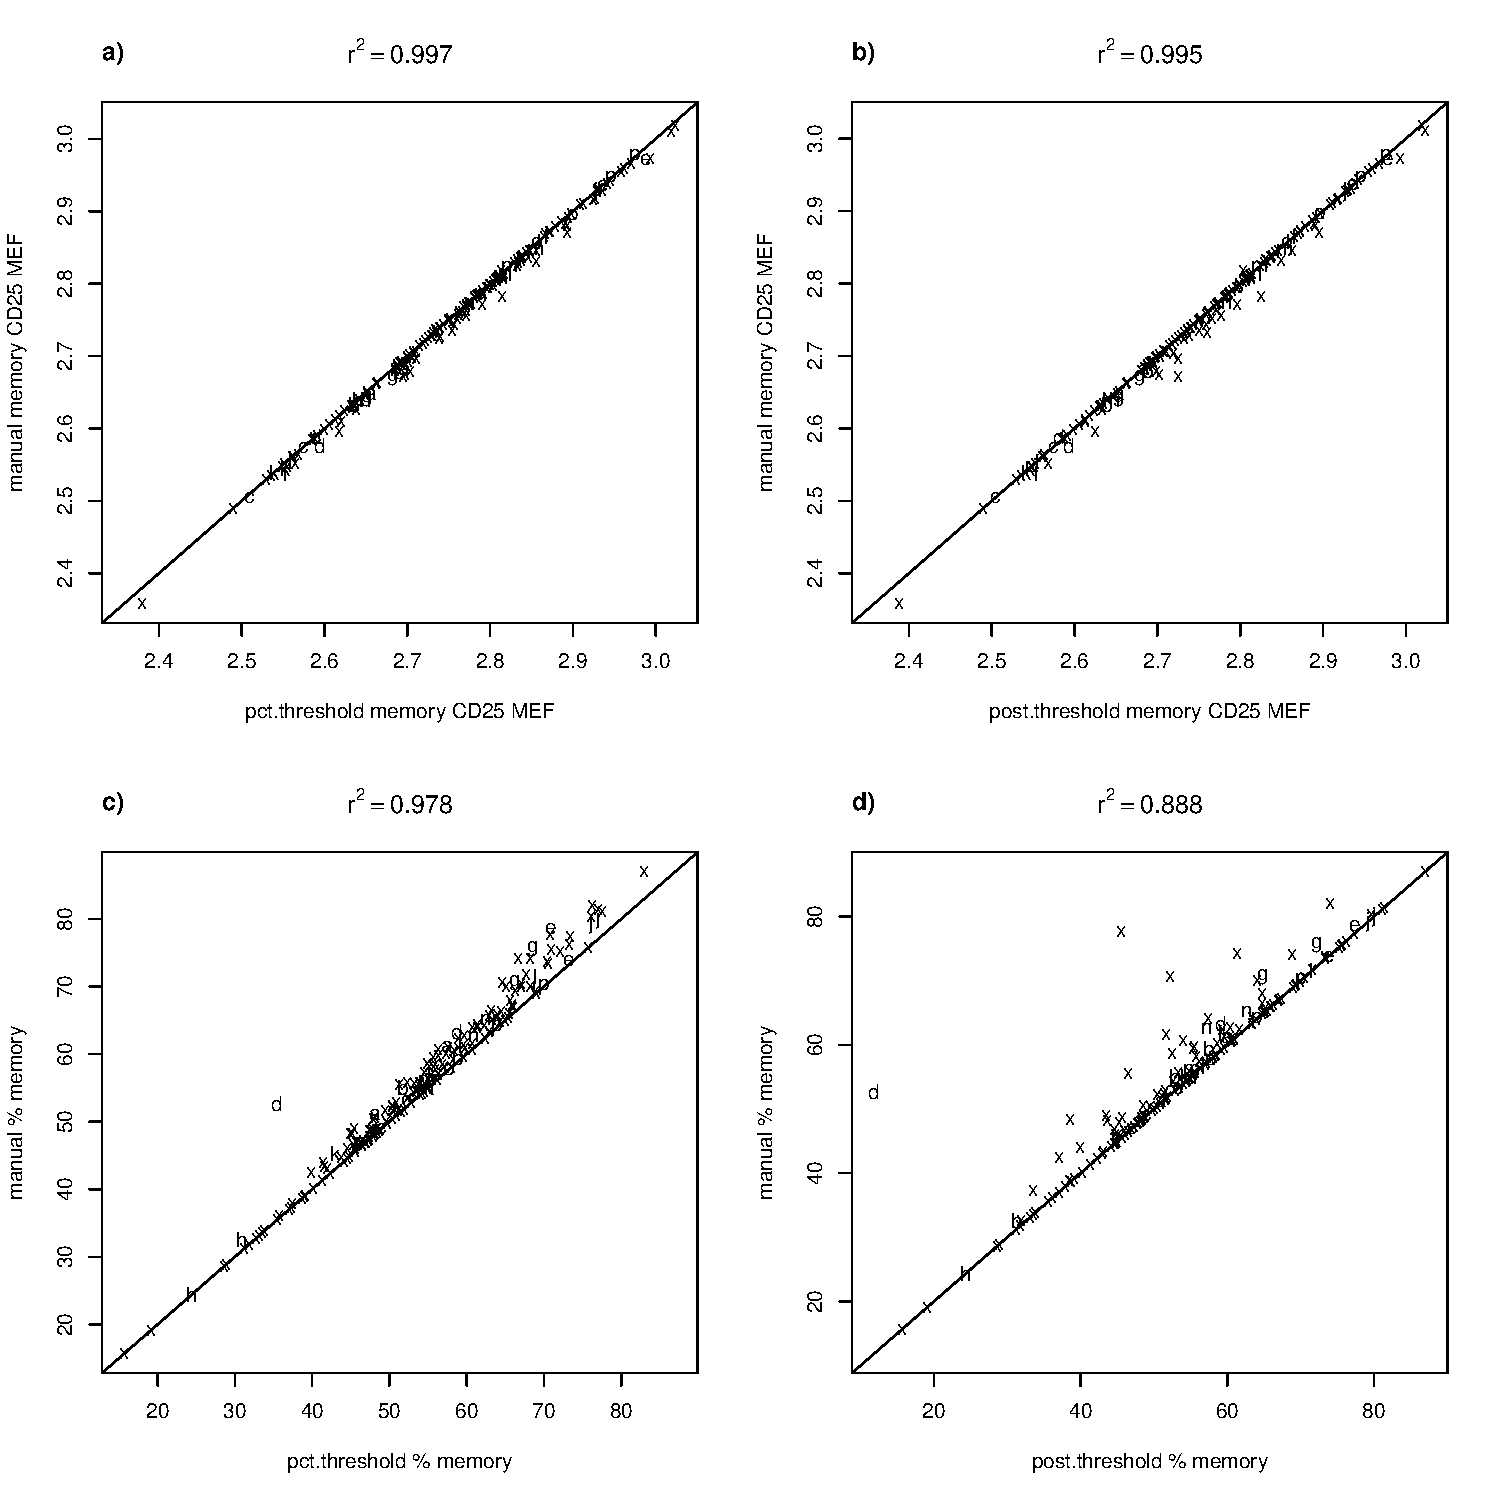
\includegraphics[scale=.6]{IL2RA/figures/memory-auto-manual-agreement-thresholds.pdf}
 %\caption{ Agreement of average daily gate positions of Gaussian mixture model method (day.thresh) with manual for MEF and for memory percentage.}
 \mycaption{figure:memory-auto-manual-agreement-thresholds}
 {Agreement of memory CD25 MEF (a and b) and percentage of memory cells (c and d), obtained from \texttt{pct.thresh} and \texttt{post.thresh} with manual.}
 {
   The agreement of memory CD25 MEF is very close to manual (a and b) while the automatic methods tend to yield smaller memory cell percentages (c and d).
 }
\end{figure} 

%%
\begin{figure}[h]
  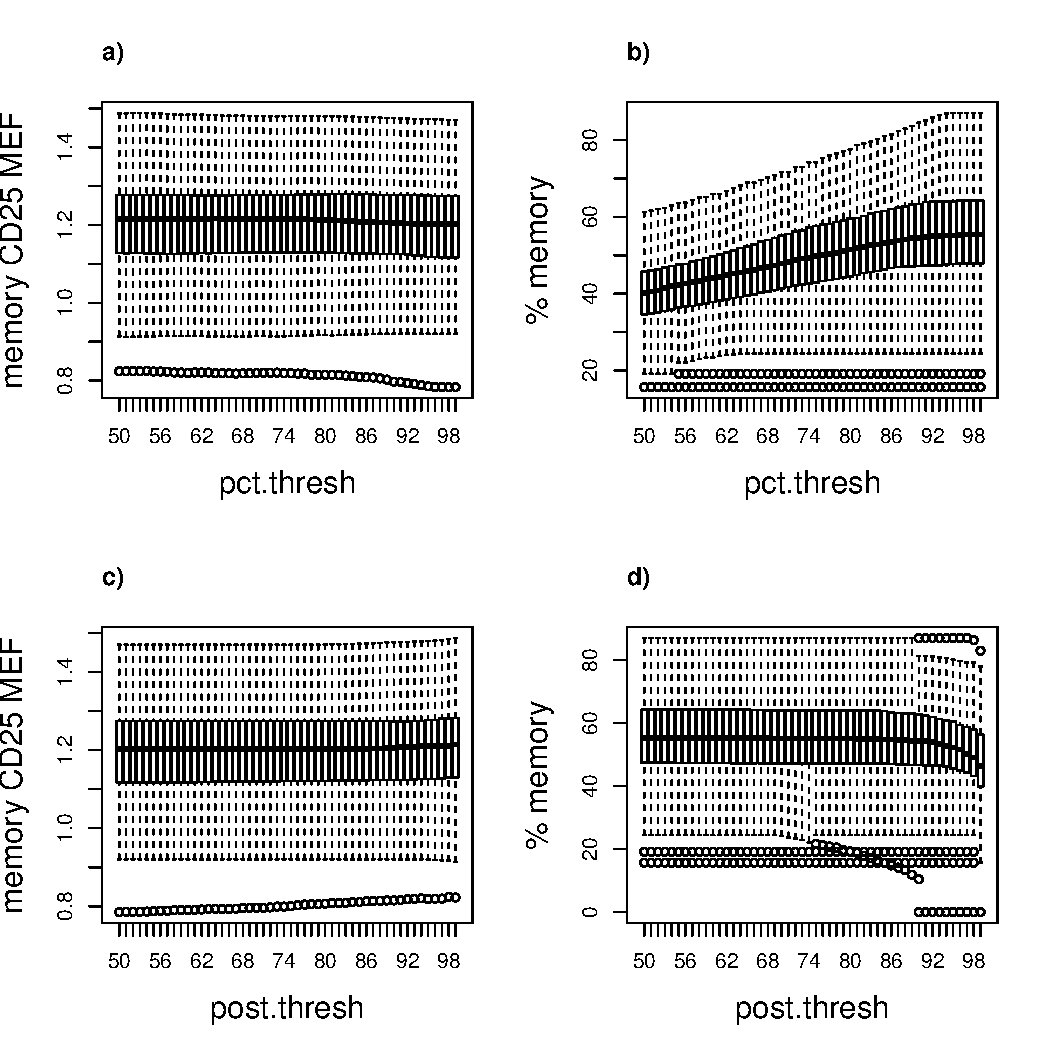
\includegraphics[width=\textwidth]{IL2RA/figures/cd45raneg-memory-gate-phenotype-sensitivity.pdf}
\mycaption{figure:cd45raneg-memory-cd25mfi}
{ Influence of threshold for \texttt{pct.thresh} and \texttt{post.thresh} on distribution of memory CD25 MEF and percent memory cell phenotypes. }
{
  Memory CD25 MEF is not sensitive to position of CD45RA gate (a and c) whereas percent memory is (b and d).
  %The distribution of memory CD25 MEF is not affected by the position of the CD45RA gate.
  On the other hand, the percent memory phenotype is more sensitive in particular when using the \texttt{pct.thresh} (c)
  method as opposed to the \texttt{post.thresh} (d).
}
\end{figure}

\begin{figure}[h]
\centering
  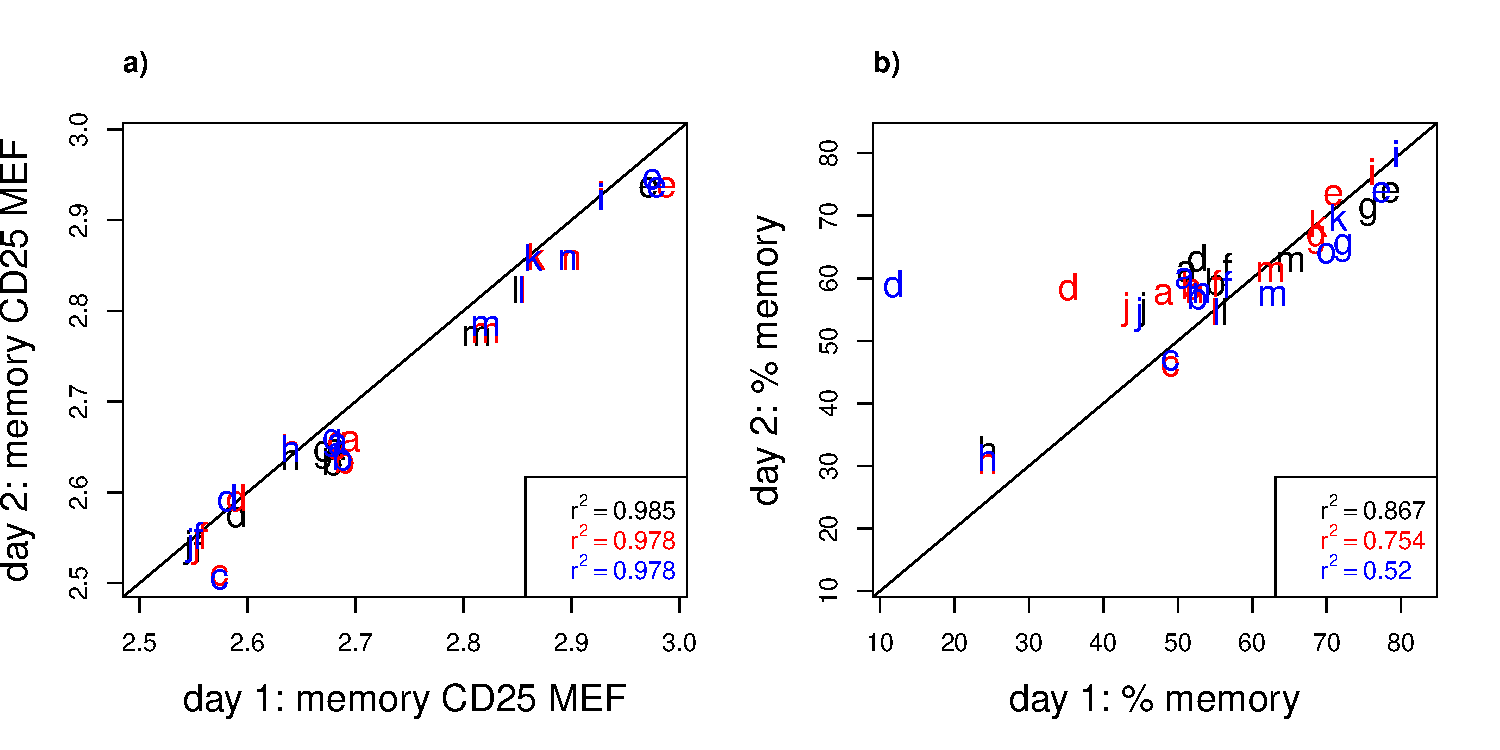
\includegraphics[width=\textwidth]{IL2RA/figures/repeatability-memory-thresholds.pdf}
\mycaption{figure:repeatability-memory-thresholds}
{Repeatability of the memory cells phenotypes, CD25 MEF (a) and percentage (b), obtained from manual gating (black), \texttt{pct.thresh} (red) and \texttt{post.thresh} (blue).}
{
  While the repeatability is very close for CD25 MEF
  ($r^2=0.985$ for manual, $r^2=0.978$ for \texttt{pct.thresh} and $r^2=0.978$ for \texttt{post.thresh})
  it varies considerably for the percentage of memory cells
  ($r^2=0.867$ for manual, $r^2=0.754$ for \texttt{pct.thresh} and $r^2=0.52$ for \texttt{post.thresh}).
  Individual d is a clear outlier when gated with the \texttt{post.thresh} method (b)

}
\end{figure}




\section{Association tests}

Having obtained cell phenotypes by different gating strategies, 
I would like to assess how these influence our association test statistics.
Since our dataset contains 15 repeated cell phenotypes from recalled individuals,
I accounted for those in my association testing 
by applying a linear mixed effects model with random intercept to allow for per individual effect.
To that purpose I used the \Rfunction{lme} from the \Rpackage{nlme}.
Each covariate, genotype, age and sex, was tested separately, with an additive recessive model assumed for the SNP effect.

Overall, the association test with the percent CD25\positive naive cells phenotype yields similar effect sizes to manual (\Cref{table:naive-cd25pos-association}).
A significant age and \snp{rs2104286} effect are reported using both manual and \texttt{beads.thresh} gating.
However, the significance of the \snp{rs2104286} effect found with \texttt{beads.thresh}, is an order of magnitude less ($10^{-4}$) than with manual ($10^{-5}$).
On the other hand, \texttt{beads.thresh} adds some evidence to the suggested association by \citet{Dendrou:2009dv} of a sex effect on percentage of CD25\positive naive cells,
whereby males have a lower percentage of naive CD25\positive than females, although the effect remains marginal.

Regarding the percentage memory cell phenotype,
an age effect is also detected using automatic methods, \texttt{post.thresh} and \texttt{pct.thresh}, however the signifcance of the association 
is an order of magnitude less with \texttt{post.thresh} (pvalue $10^{-2}$) than with manual and \texttt{pct.thresh} (pvalue $10^{-3}$).
This could be due to greater noise in the measurement as suggested by lower repeatability.
Also, noteworthy, is that a marginally significant \snp{rs2104286} effect (pvalue=$0.042322$) is reported with \texttt{post.thresh}, which is not found with the
other methods.  
However, on closer inspection, the association appears to be driven by the outlying sample from individual d (\Cref{figure:rs2104286-memory}).

For the memory CD25 MEF cell phenotype, the association results between manual and automatic are virtually identical (\Cref{table:memory-cell-mef-effect}),
which is to be expected, given this cell phenotype is largely unchanged by the CD45RA gate position (\Cref{figure:cd45raneg-memory-cd25mfi}).

%Note that the original results from \citet{Dendrou:2009dv}, which are summarised in \Cref{table:calli-results},
%do not match: the repeatability and the p-values are not exactly reproducible.
%I believe this is largely due to technical discrepancies between the gating done in FlowJo and the
%analysis done in R using the exported FCS and gate files.
%However, the analysis I conducted in this chapter is consistent across all samples.



\begin{table}[h]
\centering
\begin{tabular}{lrrr}
\rowcolor{Gray}
\snp{rs12722495} & effect & 95\%CI          & p-value\\
manual           & -2.479  & [-5.422;0.463]  & 0.098145\\
beads.thresh       & -1.509  & [-4.453;1.435]   & 0.31326\\
\rowcolor{Gray}
\snp{rs2104286}  & effect & 95\%CI          & p-value\\
manual           & -4.714  & [-6.894;-2.534]  & \textcolor{red}{3.2017e-05}\\
beads.thresh       & -4.39  & [-6.569;-2.212]   & \textcolor{red}{0.0001014}\\
\rowcolor{Gray}
\snp{rs11594656} & effect & 95\%CI          & p-value\\
manual           & -1.459  & [-3.924;1.006]  & 0.2443\\
beads.thresh       & -1.328  & [-3.774;1.118]   & 0.28531\\
\rowcolor{Gray}
Age              & effect & 95\%CI          & p-value\\
manual           & 0.475  & [0.286;0.664]  & \textcolor{red}{1.6584e-06}\\
beads.thresh       & 0.457  & [0.269;0.645]   & \textcolor{red}{3.514e-06}\\
\rowcolor{Gray}
Sex              & effect & 95\%CI          & p-value\\
manual           & -4.216  & [-7.856;-0.575]  & \textcolor{red}{0.023475}\\
beads.thresh       & -4.327  & [-7.936;-0.718]   & \textcolor{red}{0.019046}\\
\end{tabular}
\mycaption{table:naive-cd25pos-association}
{Genotype, age and sex effect sizes on percentage of \protein{CD25}\positive cells.}
{
Effect of \snp{rs12722495}, \snp{rs2104286}, \snp{rs11594656}, age and sex,
on the percentage of \protein{CD25}\positive naive cells.
}
\end{table}

\begin{table}[h]\footnotesize
\centering
\begin{tabular}{lrrr}
\rowcolor{Gray}
\snp{rs12722495} & effect & 95\%CI         & p-value\\
manual           & 0.062  & [0.036;0.088]  & \textcolor{red}{4.7176e-06}\\
pct.thresh       & 0.06   & [0.034;0.086]  & \textcolor{red}{9.0361e-06}\\
post.thresh      & 0.061  & [0.035;0.087]  & \textcolor{red}{6.822e-06}\\
\rowcolor{Gray}
\snp{rs2104286}  & effect & 95\%CI         & p-value\\
manual           & 0.014  & [-0.007;0.035] & 0.18022\\
pct.thresh       & 0.014  & [-0.007;0.035] & 0.19525\\
post.thresh      & 0.014  & [-0.007;0.035] & 0.18634\\
\rowcolor{Gray}
\snp{rs11594656} & effect & 95\%CI         & p-value\\
manual           & 0.012  & [-0.011;0.035] & 0.29945\\
pct.thresh       & 0.011  & [-0.012;0.034] & 0.34754\\
post.thresh      & 0.011  & [-0.012;0.033] & 0.35147\\
\rowcolor{Gray}
Age              & effect & 95\%CI         & p-value\\
manual           & 0.001  & [-0.001;0.003] & 0.43937\\
pct.thresh       & 0.001  & [-0.001;0.003] & 0.44201\\
post.thresh      & 0.001  & [-0.001;0.003] & 0.38071\\
\rowcolor{Gray}
Sex              & effect & 95\%CI         & p-value\\
manual           & 0      & [-0.034;0.034] & 0.9983\\
pct.thresh       & 0.001  & [-0.033;0.035] & 0.95584\\
post.thresh      & 0.002  & [-0.032;0.036] & 0.89534\\
\end{tabular}
\mycaption{table:memory-cell-mef-effect}
{Memory CD25 MEF effect sizes.}
{
Effect of \snp{rs12722495}, \snp{rs2104286}, \snp{rs11594656}, sex and age on memory CD25 MEF.
}
\end{table}


\begin{table}[h]\footnotesize
\centering
\begin{tabular}{lrrr}
\rowcolor{Gray}
\snp{rs12722495} & effect & 95\%CI         & p-value\\
manual           & 1.736  & [-1.246;4.718] & 0.25209\\
pct.thresh       & 2.326  & [-0.408;5.06]  & 0.094952\\
post.thresh      & 2.624  & [-0.26;5.508]  & 0.074263\\
mm               & 1.131  & [-1.84;4.101]  & 0.45366\\
spmm             & 1.957  & [-1.301;5.214] & 0.23746\\
\rowcolor{Gray}
\snp{rs2104286}  & effect & 95\%CI         & p-value\\
manual           & 1.75   & [-0.544;4.045] & 0.13399\\
pct.thresh       & 2.051  & [-0.063;4.165] & 0.057164\\
post.thresh      & 2.337  & [0.082;4.593]  & \textcolor{red}{0.042322}\\
mm               & 1.118  & [-1.194;3.431] & 0.34129\\
spmm             & 1.775  & [-0.744;4.293] & 0.16611\\
\rowcolor{Gray}
\snp{rs11594656} & effect & 95\%CI         & p-value\\
manual           & -0.018 & [-2.514;2.479] & 0.98884\\
pct.thresh       & 0.269  & [-2.048;2.585] & 0.81927\\
post.thresh      & 0.402  & [-2.092;2.896] & 0.75075\\
mm               & 1.253  & [-1.265;3.771] & 0.32737\\
spmm             & 1.272  & [-1.466;4.01]  & 0.36044\\
\rowcolor{Gray}
Age              & effect & 95\%CI         & p-value\\
manual           & 0.387  & [0.192;0.582]  & \textcolor{red}{0.000127}\\
pct.thresh       & 0.35   & [0.169;0.531]  & \textcolor{red}{0.00018575}\\
post.thresh      & 0.316  & [0.119;0.513]  & \textcolor{red}{0.0018033}\\
mm               & 0.431  & [0.236;0.625]  & \textcolor{red}{2.0985e-05}\\
spmm             & 0.534  & [0.326;0.743]  & \textcolor{red}{1.0325e-06}\\
\rowcolor{Gray}
Sex              & effect & 95\%CI         & p-value\\
manual           & 3.485  & [-0.198;7.168] & 0.063526\\
pct.thresh       & 2.826  & [-0.594;6.246] & 0.10471\\
post.thresh      & 2.811  & [-0.86;6.481]  & 0.1325\\
mm               & 2.793  & [-0.925;6.51]  & 0.13998\\
spmm             & 3.361  & [-0.687;7.408] & 0.10308\\
\end{tabular} 
\mycaption{table:memory-cell-pct-effect}
{Memory percentage effect sizes.}
{
Effect of \snp{rs12722495}, \snp{rs2104286}, \snp{rs11594656}, sex and age on memory cell percentage.
}
\end{table}


\begin{figure}[h]
\centering
\begin{subfigure}[b]{.4\textwidth}
    \centering
    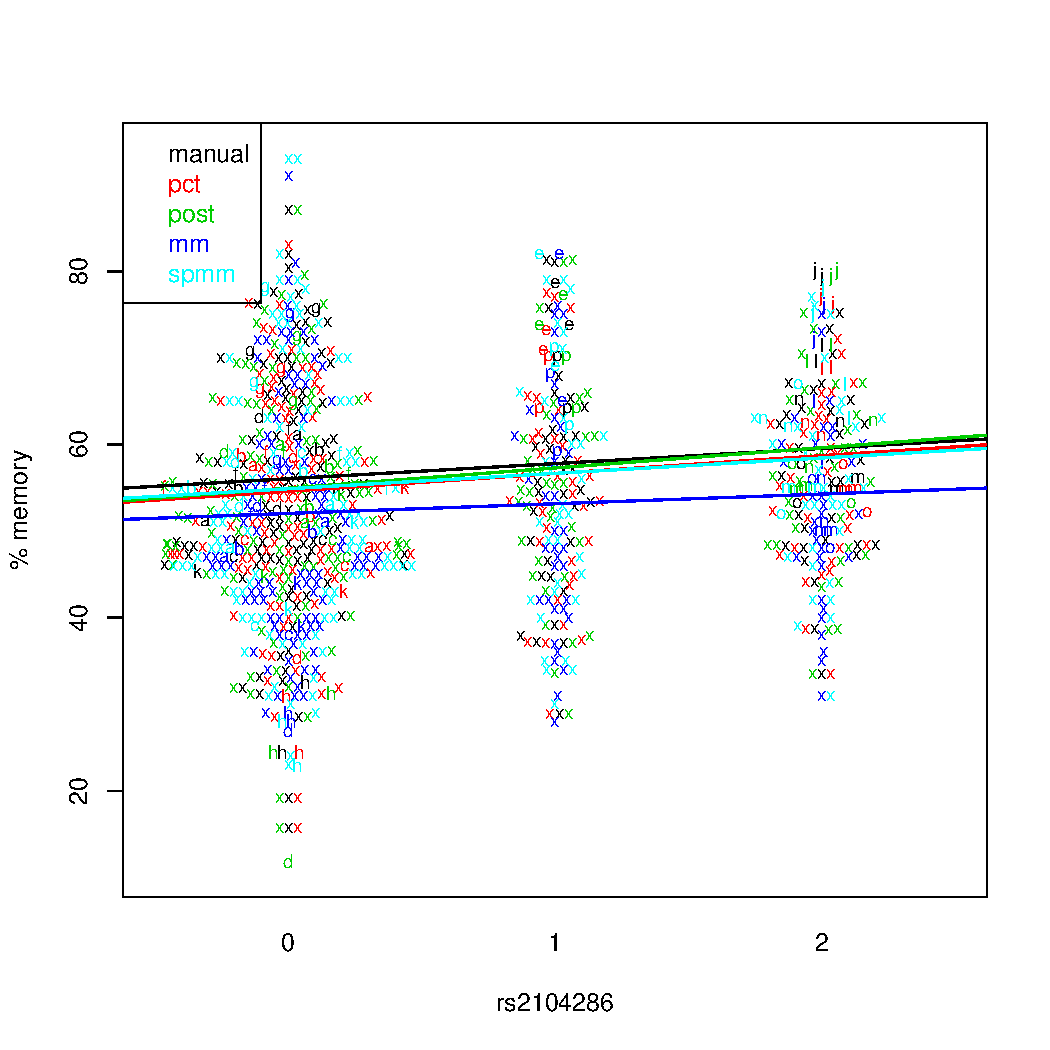
\includegraphics[scale=.35]{IL2RA/figures/rs2104286-ratio.pdf}
    \caption{}
\end{subfigure}
~
\begin{subfigure}[b]{.4\textwidth}
    \centering
    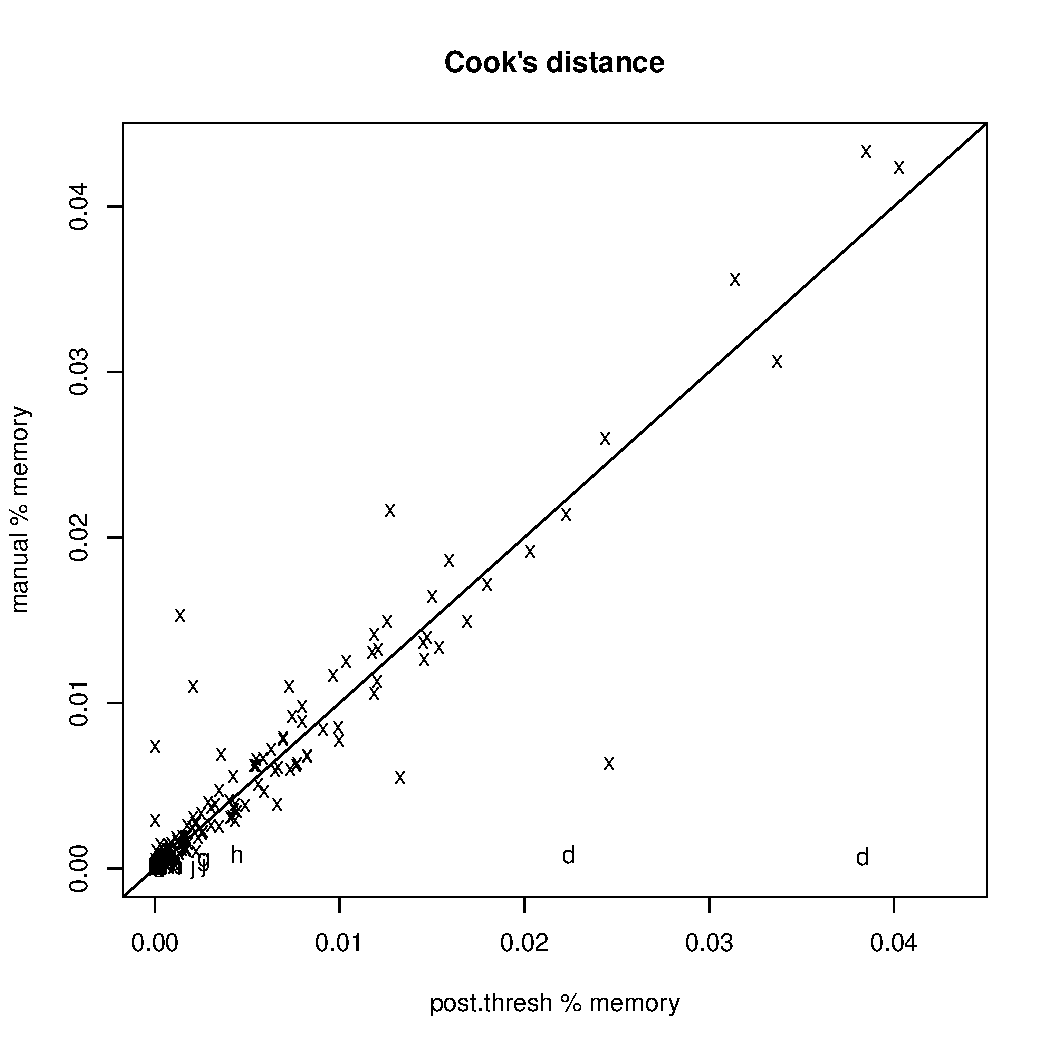
\includegraphics[scale=.35]{IL2RA/figures/rs2104286-ratio-cooks-distance.pdf}
    \caption{}
\end{subfigure}
\mycaption{figure:rs2104286-memory}
{Effect of rs2104286 on percent memory gated by manual (black), \texttt{post.thresh} (green) and \texttt{pct.thresh} (red).}
{
  In \Cref{table:memory-cell-pct-effect}, marginally significant association is detected with \snp{rs2104286}.
  This is due to the leverage of individual d which stands out as an outlier (b).
}
\end{figure}



\clearpage


%%% DISCUSSION
\section{Discussion}

%A more real challenge however is to do with the nature of flow data.
%Noise or unexplained variation is inherent to all technologies and the signal to noise ratio in flow cytometry can vary greatly depending on the sample,
%the experimental protocol and the instrument.
%Even when running a "clean" sample such as beads which are manufactured to be identical on a well calibrated instrument the signal to noise ratio of the resulting bead populations is never greater than 30.
%In biological samples the level of noise is much higher and so is the number of outliers which contribute to confusing automatic methods,
%especially when in most cases the number of clusters is unknown and needs to be estimated from the ratio of explained to unexplained variance in the data.
%Many clustering solutions have been suggested as part of the Bioconductor suite of packages which adopt different approaches to trying to solve this problem.
%But remains the problem of how to benchmark these various solutions: comparison to manual gating, correlation with clinical outcome?
%One criteria we have suggested and tested is that of repeatability of results derived from stable features in samples from the same healthy individual recalled up to 7 months later. (Spidlen et al., 2010).
%
In this chapter, I have shown that bead data is readily gated by automatic methods and that the results are comparable to manual gating.
Automatic gating of bead data is fast and automates other related tasks such as MFI to MEF transformation, and threshold selection.
%and reporting of instrument properties such as the detection threshold or the signal-to-noise ratio (or coefficient of variation).

Gating of biological data is more difficult as we have little prior knowledge of the sample we are analysing and the data is far more noisy.
So far, I have developed two automatic univariate gating strategies:
\begin{itemise}
\item a bead defined threshold method on \protein{CD25} to identify CD25\positive naive cells
\item a two component mixture model on \protein{CD45RA} to identify memory cells (CD45RA\negative)
\end{itemise}

My \protein{CD25} univariate gating method (\texttt{beads.thresh}) relies on defining a threshold based on automatically gated bead data.
The value of the threshold is selected as the percentile of the blank bead population which mimimises the mean squared difference with manual gate positions.
The percentage of naive \protein{CD25}\positive cells phenotype identified with my approach showed better repeatability than manual (\Cref{figure:repeatability-cd25pos-naive}).
My approach defines one threshold for all samples gated on the same day,
%which seems appropriate given the blank bead population yields the detection threshold of the instrument on that day.
whereas the manual approach, relies on isotype controls and allows for different thresholds per day.
Isotype controls should theoretically be an estimate of background but have been criticised for being an extra source of noise \citep{OGorman:1999vd,Maecker:2006ft}.

My \protein{CD45RA} univariate gating method fits a specific model to the data: a mixture of two univariate distributions.
The parameters of the model are estimated using an \Gls{EM} algorithm \citep{Dempster:1977ul} initialised with K-medoids.

In a first instance, I used the parameters estimated by the two-component mixture model.
Specifically, I used the weight parameter of the first component as the percentage of memory cells phenotype.
%Additionally to the mixture of two univariate Gaussian model (\texttt{mm}), I also applied a more flexible model of two symmetric kernel density estimates (\texttt{spmm}).
Although this seemed a sensible approach from the statistical perspective of fitting a two-component mixture model, it does not match the biological perspective that transitional
cells should be excluded.

Therefore, in the second instance, I attempted to emulate manual gating by defining a threshold.
I tried two approaches of defining a threshold, \texttt{pct.thresh} which thresholds on the percentile of the first component of the fitted mixture model,
and \texttt{post.thresh} which thresholds instead on the posterior probability of the first component.
As with the \texttt{beads.thresh}, the value of the threshold is selected as the value which mimimises the \gls{MSD} with manual gate positions.
%In the future it may be interesting to use all cells and average over the posterior probabilities.
%I have found however that there is sometimes an upper bound to the posterior probability
%However, if the model does not fit the data then it is unlikely that the position of the gate will be sensible, which may give rise to outliers.

Two benchmarks were used to evaluate my univariate gating strategies: repeatability and comparison of the effects sizes obtained 
by \citet{Dendrou:2009dv} using manual.

Repeatability is an independent measure which does not require comparison to other gating methods (such as manual).
Unfortunately, given that in our data set only 15 samples are repeated, it is difficult to evaluate methods on such a small sample size.
Moreover, good repeatability does not necessarily imply that the gating is unbiased but rather that the gating is consistent.
Hence repeatability, needs to be complemented with some metric, in the form of manual gating or some prior biological knowledge,
to assess whether the computed cell phenotypes are in a sensible range.

I have shown that the difference in the identification of cell phenotypes by different gating methods can influence the effect size estimates in association studies.
In particular, outliers can have an important influence in relation to their leverage as seen in \Cref{figure:rs2104286-memory}.
For example when testing association with age, outlier cell phenotypes from younger or older individuals have more leverage than ones closer to the mean.
When testing for association with genotype, outlier cell phenotypes from rarer variants have more leverage than one from common variants.

%\paragraph{Outlier Detection Metric}
Hence, if we are to deploy automatic gating techniques more generally, detection of outliers is crucial, to avoid false positive associations.
In particular, we require outlier detection metrics which do not only rely on the availability of repeated samples or manual gates.
Already, we have seen that looking at the maximum posterior probability in a sample can give us some insight (\Cref{figure:cd45ra-posterior-threshold-fail}).
Another metric of evaluating how well a model fits the data could be a cost function like the \gls{MISE}.
I will revisit outlier metrics in the next two chapters.

When outliers have been detected, we may want to exclude or down-weight them, or extend the gating method to account for these.
One simple way of modifying the method, could be to use the gate positions in non-outlier samples to influence that in outliers.
This could motivate borrowing information from other samples, using for example a hierarchical Bayesian framework as was recently developed by \citet{Cron:2013dh}.

However, one may argue that this approach, conceals rather than addresses the underlying problem of poor model fit.
For example, as we see from the trimodal distribution in \Cref{figure:cd45ra-threshold-example},
it may be more appropriate to fit a three component instead of a two component mixture model on this sample.

So far, MFI to MEF using beads has been automated but there are still many parts of the process left to be automated.
In the next chapter, I will develop a modular pipeline to further automate the analysis of flow cytometry data generated by our lab.
It will be possible to plug in different types of transformations and gating strategies and see how this influences
the results of the analysis.
This should encourage the wider use of automatic analysis methods for flow data.

%Chris points:
%Manual gating could be applied in a subset of samples and then auto gating could use that info to guide the gating.
%This provides reassurance to gaters that their rules are follow.  Manual gaters may not always be keen to relinquish control
%to a computer: seeing is believing.


%\paragraph{Discovering New Subsets of Interest with Automatic Methods}
%So far in this chapter, I have only considered the cell phenotypes defined by \citet{Dendrou:2009dv}.
%In general, these cell populations may not necessarily represent true clusters but are established cells of interest within the field of immunology
%which are known to express \protein{CD25} and hence hypothesised to associate with \gene{IL2RA} SNPs.
%Potentially, there might exist other \protein{CD25} cell phenotypes than the ones under study which also correlate well with these SNPs.
%These might only be separable in higher dimensional space.
%These could be identifiable using unsupervised methods which find clusters in one or more dimensions when the number of clusters is unknown.
%Similar work has been undertaken by \citet{Aghaeepour:2012fq} in identifiying novel subsets which correlate with a clinical outcome in HIV patients.
%Fealect (?) is a method of choosing features of these cells subsets which best correlate with the response variable.

%\paragraph{An Internal Automatic Pipeline}


%The pipeline will be configurable to so account for the wealth Obviously the type of analysis will be dependent on the experiment but it may be possible 
%One of the reasons for this is simply that the analysis requirements for different types of flow experiments are so varied that it is difficult to design a solution which will service all needs.


%% TODO
%This clearly rests on the assumption that in the majority of samples, the position of the gate is correct.
%I tried this approach with \texttt{day.thresh} by averaging gates on non-outlier samples and applying these to the outlier samples.
%thus exploiting day effects
%A more formal approach could be to extend this by using some outlier metric to define weights so that \texttt{day.thresh} leans more heavily
%towards samples where the model fits better.
%We have seen that one way of improving overall gating is to allow for the gate positions on well-gated samples to influence those of badly-gated ones.
%Clearly, the implicit assumption with \texttt{day.thresh} and outlier detection in general, is that there are enough well-gated samples to positively influence the gate position of the ill-gated ones
%and that the gates in outlier samples should be in about the same position since the sample is noisy but not fundamentally different.  
%One reason why the manual gates on that day are more appropriate is because a human uses prior knowledge obtained from other samples of where the gates should lie.
%A first attempt at learning from other samples (\texttt{day.thresh}) is to compute the mean of the position of the CD45RA gates defined by the \texttt{pct.thresh}
%method across all samples from the same day excluding the outlying sample from individual d on day one.
%Similar to the threshold method for \protein{CD25}\positive covered in the previous section, we now have a fixed gate for all samples analysed on the same day.
%The \texttt{day.thresh} agreement with manual is improved over x but not as good as y
%%but this time requires estimation of gate position by mm followed by averaging their position.
%%When attempting to gate more noisy samples, a manual gater will maybe use other samples as a reference.
%%One way of better gating is to use prior knowledge from other samples from the same day where the repeatability is good.
%Since the gate position is less sensitive to outlier samples, \texttt{day.thresh} improves overall repeatability (\Cref{figure:repeatability-memory-thresholds-learned}) compared to \texttt{pct.thresh}.  
%Nonetheless, manual still achieves higher repeatability (\Cref{table:repeatability-results}) as
%the gater has prior knowledge of cell population frequencies when dealing with outliers.
%


